% Initial System Characterization

\documentclass[9pt]{article} % use larger type; default would be 10pt

\usepackage[utf8]{inputenc} % set input encoding (not needed with XeLaTeX)
\usepackage{amsmath}
\usepackage{graphicx}
\usepackage{multicol}
\setlength{\columnsep}{0.5cm}
\usepackage[backend=biber]{biblatex} %, style=apa
\usepackage[margin=1.0in]{geometry}
\usepackage{siunitx}
\addbibresource{references.bib}

% For two figures side-by-side
\usepackage{mwe}
\usepackage[font=small]{caption}


\numberwithin{equation}{section} % number within sections
% \usepackage[parfill]{parskip} % new line without indent

%%% Examples of Article customizations
% These packages are optional, depending whether you want the features they provide.
% See the LaTeX Companion or other references for full information.

%%% PAGE DIMENSIONS
\usepackage{changepage} % to adjust margins for a single paragraph
\usepackage{geometry} % to change the page dimensions
\geometry{a4paper} % or letterpaper (US) or a5paper or....
% \geometry{margin=2in} % for example, change the margins to 2 inches all round
% \geometry{landscape} % set up the page for landscape
%   read geometry.pdf for detailed page layout information

\usepackage{graphicx} % support the \includegraphics command and options

\graphicspath{ {./sim_files/}{./cad_files/} }

% \usepackage[parfill]{parskip} % Activate to begin paragraphs with an empty line rather than an indent

%%% PACKAGES
\usepackage{booktabs} % for much better looking tables
\usepackage{array} % for better arrays (eg matrices) in maths
\usepackage{paralist} % very flexible & customisable lists (eg. enumerate/itemize, etc.)
\usepackage{verbatim} % adds environment for commenting out blocks of text & for better verbatim
\usepackage{subfig} % make it possible to include more than one captioned figure/table in a single float
% These packages are all incorporated in the memoir class to one degree or another...

%%% HEADERS & FOOTERS
\usepackage{fancyhdr} % This should be set AFTER setting up the page geometry
\pagestyle{fancy} % options: empty , plain , fancy
\renewcommand{\headrulewidth}{0pt} % customise the layout...
\lhead{}\chead{}\rhead{}
\lfoot{}\cfoot{\thepage}\rfoot{}

%%% SECTION TITLE APPEARANCE
\usepackage{sectsty}
\allsectionsfont{\sffamily\mdseries\upshape} % (See the fntguide.pdf for font help)
% (This matches ConTeXt defaults)

%%% ToC (table of contents) APPEARANCE
\usepackage[nottoc,notlof,notlot]{tocbibind} % Put the bibliography in the ToC
\usepackage[titles,subfigure]{tocloft} % Alter the style of the Table of Contents
\renewcommand{\cftsecfont}{\rmfamily\mdseries\upshape}
\renewcommand{\cftsecpagefont}{\rmfamily\mdseries\upshape} % No bold!

%%% TITLE APPEARANCE (custom)
\usepackage[affil-it]{authblk} 
\usepackage{etoolbox}
\usepackage{lmodern}
%\usepackage{titling}
\makeatletter
\patchcmd{\@maketitle}{\LARGE \@title}{\fontsize{17}{20.2}\selectfont\@title}{}{}
\makeatother
\renewcommand\Authfont{\fontsize{12}{14.4}\selectfont}
\renewcommand\Affilfont{\fontsize{10}{12.8}\itshape}
\makeatletter
\renewcommand\AB@affilsepx{, \protect\Affilfont}
\makeatother

\usepackage{dblfnote} % multicolumn footnotes

%%% END Article customizations

%%% The "real" document content comes below...
\title{Development of a Cost-Effective 1.5kN Liquid-Fueled Rocket Propulsion System}
\author[1]{Jason Chen \footnote{jay.chen135@gmail.com, contact@projectcaelus.org}}
\affil[1]{Project Lead and Chief Engineer}
\author[2]{Srikar Gouru \footnote{srikarg89@gmail.com}}
\affil[2]{Flight and Ground Software Lead}
\author[3]{Sophia Troshynski \footnote{stroshynski@gmail.com}}
\affil[3]{Manufacturing Lead}
\author[4]{Ron Nachum \footnote{ronnachum13@gmail.com}}
\affil[4]{Propulsion Lead}
\author[5]{Ankit Khandelwal \footnote{amtron521@gmail.com}}
\affil[5]{Avionics Lead}
\author[6]{Ethan Ai \footnote{ethanai22@gmail.com}}
\affil[6]{CAD and Testing Lead}
\author[7]{Dabini Muldoon \footnote{cdabinim2249@gmail.com}}
\affil[7]{Structures and Ground Operations Lead}
\date{} % Activate to display a given date or no date (if empty), otherwise the current date is printed
\begin{document}
\maketitle
\vspace{-1cm}
\begin{center}
\centering

\includegraphics[scale=0.5, width=0.175\textwidth]{caelus_logo}

Project Caelus, 501(c)(3)

(Initial revision 06 August, 2019; received 26 March, 2020)
\end{center}

%%% ABSTRACT
\begin{adjustwidth}{40pt}{40pt}
\hspace{\parindent} This is an example of the abstract. Mit der CNN.com Europe Edition verfügt der TV-Sender CNN über eine umfassende Webseite, die im Minutentakt rund um die Uhr aktualisierte Weltnachrichten aus einer europäischen Perspektive auf den Bildschirm bringt. Wichtige, globale Ereignisse, geordnet in den Rubriken breaking news, current news headlines oder in depth, werden mit Hilfe von Video- und Audioclips, Bildern, Karten, Profilen, Zeitachsen und Tatsachenberichten fundiert dargestellt. Die Nachrichten stützen sich auf die Expertenanalysen der CNN Korrespondenten. Die Berichte verweisen auf andere relevante CNN Reportagen und zu Meldungen anderer Websites. Zusätzlich besteht die Möglichkeit, Videos anzufordern und mittels einer Suchfunktion Zugriff auf bereits gesendete Berichte und gesonderte Themenbereiche, die seit 1995 bearbeitet wurden, zu erhalten.

\end{adjustwidth}
\vspace{0.4cm}
\section{Nomenclature} \label{sec: nomenclature}
\vspace{0.1cm}
%\begin{center}
\begin{tabular}{lll}
\textbf{Symbols} \\ 
$\epsilon$ & = \quad Expansion ratio & $$ \\
$\gamma$ & = \quad Ratio of specific heats & $$ \\
$\rho$ & = \quad Density & $g/cm^{3}$ \\
$C^{*}$ & = \quad Characteristic velocity & $m/s$ \\
$C_{d}$ & = \quad Discharge coefficient & $$ \\
$C_{v}$ & = \quad Valve flow coefficient & $$ \\
$f_{d}$ & = \quad Friction factor & $$ \\
$F_{t}$ & = \quad Thrust & $N$ \\
$g_{0}$ & = \quad Acceleration due to gravity & $m/s^{2}$ \\
$I_{sp} $ & = \quad Specific impulse & $s$ \\
$\dot{m}$ & = \quad Mass flow rate & $kg/s$ \\
$O/F$ & = \quad Oxidizer-to-fuel ratio & $$ \\
$Q $ & = \quad Volumetric flow rate & $L/s$ \\
\end{tabular} 
\begin{tabular}{ll}
\textbf{Acronyms} \\ 
$CEA $ & = \quad Chemical equilibrium \\ 
$ $ & \qquad \enskip with applications \\
$COTS $ & = \quad Commercial off-the-shelf \\
$DAQ $ & = \quad Data acquisition \& control \\
$FOD $ & = \quad Foreign object debris \\
$GLOW $ & = \quad Gross lift-off weight \\
$MECO$ & = \quad Main engine cut-off \\
$P\&ID $ & = \quad Plumbing and \\
$ $ & \qquad \enskip instrumentation diagram\\
$PT $ & = \quad Pressure transducer \\
$TC $ & = \quad Thermocouple \\
$SF $ & = \quad Safety factor \\
$VDC $ & = \quad Direct current voltage \\
\end{tabular} 
\vspace{0.2cm} \newline
%\end{center}
Note: Subscripts follow the convention outlined in \cite{rpe}. Unless otherwise specified, subscript $0$ indicates at stagnation or impact conditions, $1$ indicates conditions at the nozzle inlet or combustion chamber, $t$ indicates the nozzle throat, $2$ is at the nozzle exit, and $3$ is at ambient conditions.

%\begin{multicols}{2}
\section{Initial System Characterization}
\hspace{\parindent}  Project Caelus' unique position as a 501(c)(3) non-profit organization consisting entirely of high school students has laid the foundation for a design approach fully committed to cost-effectiveness, simplicity, and reliability. The following section outlines the initial design choices made for our overall system and reflects our emphasis on the aforementioned ideals.
\subsection{Objectives}
The Callisto 1 system is set to the following constraints and objectives:
\begin{enumerate}
\item Reach an altitude of 1500 m ($\approx$ 5000 ft).
\item A $GLOW$ of no more than 30 kg ($\approx$ 70 lbsm).
\item A nominal main engine thrust of 1.5 kN ($\approx$ 350 lbsf).
\item A chamber pressure in the range of around 15 Bar to 20 Bar ($\approx$ 218 psi to 300 psi)
\item Consume a budget of no more than \$10,000 USD.
\item Utilize $95\%$ ethyl alcohol and nitrous oxide as the propellant combination.
\end{enumerate}

\begin{figure}
    \centering
    \begin{minipage}{0.475\textwidth}
        \centering
        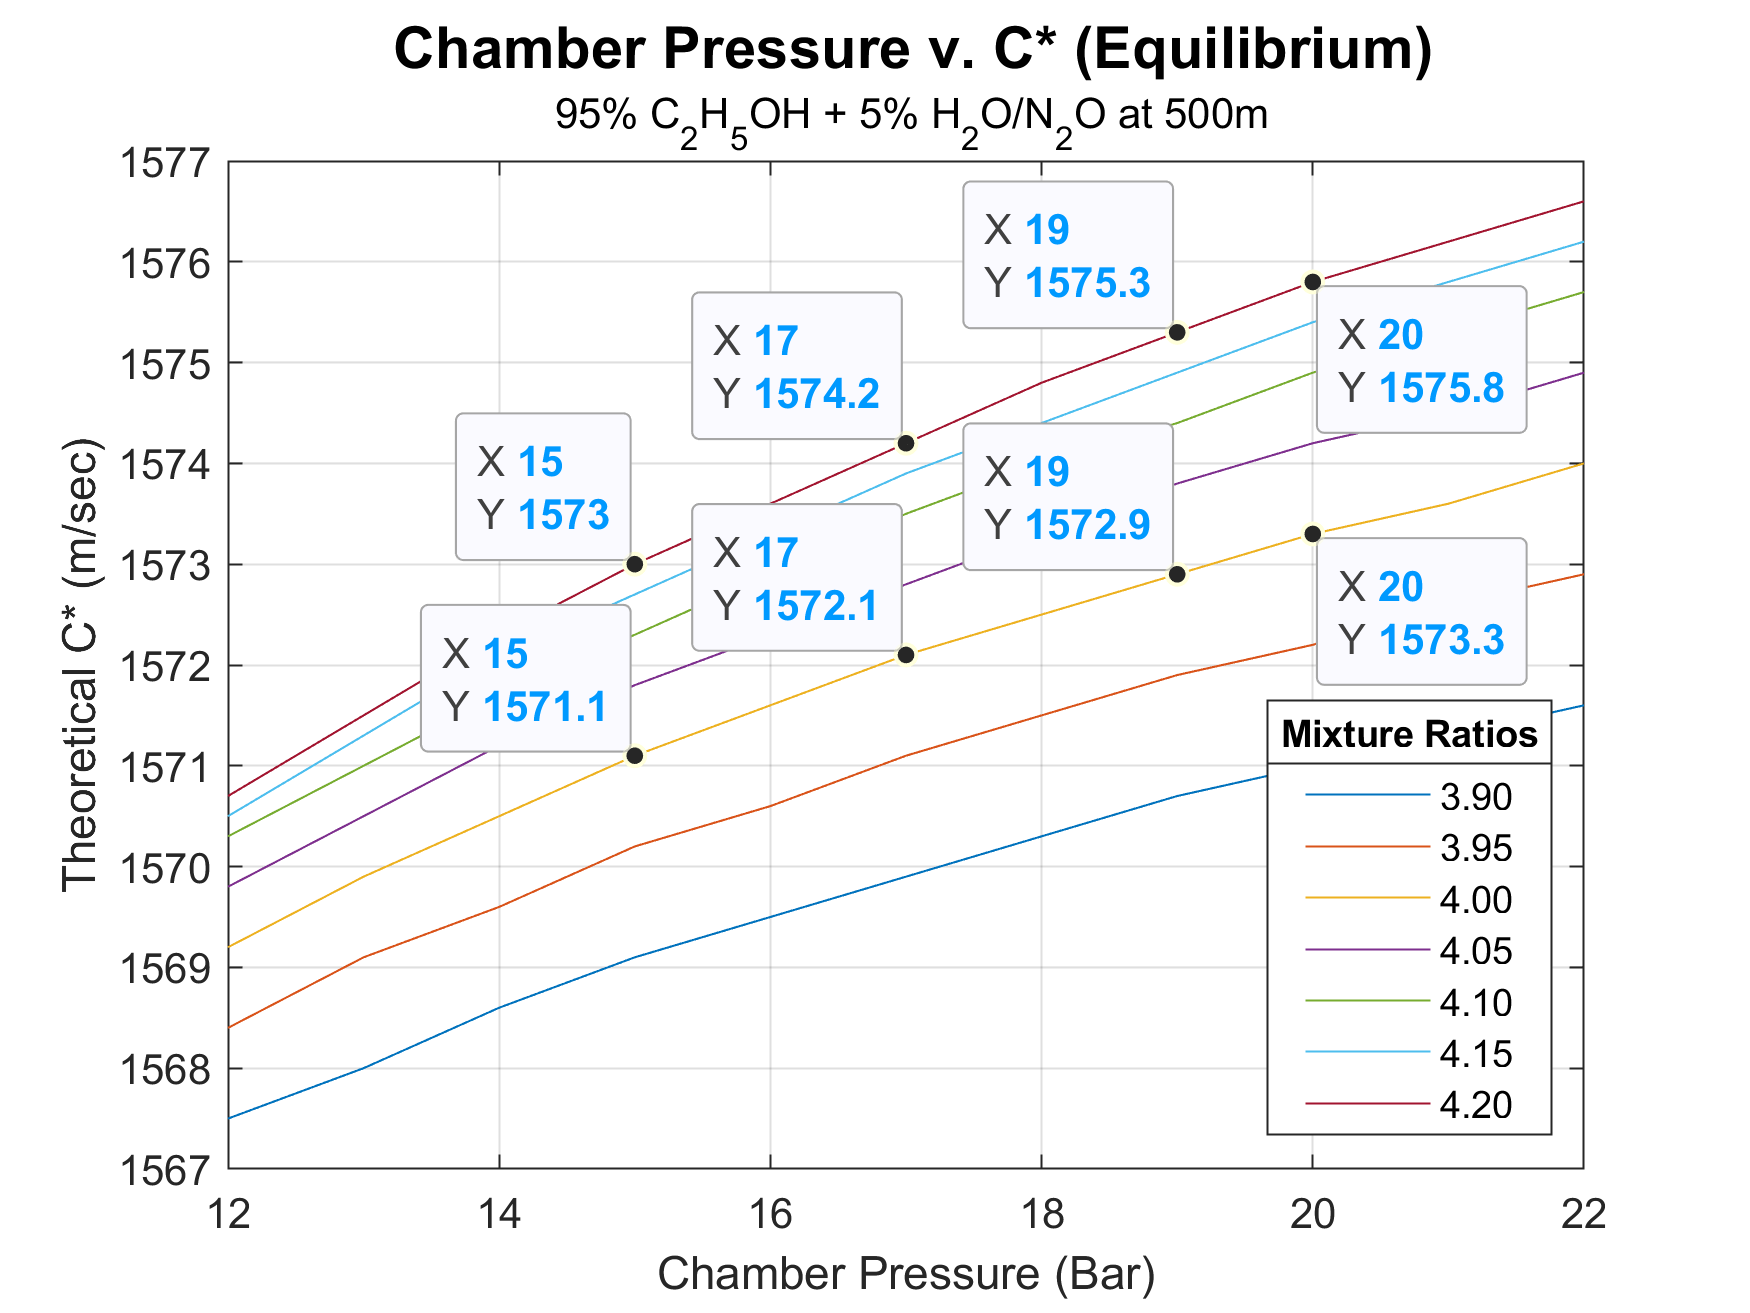
\includegraphics[scale=0.5, width=0.9\textwidth]{cp_cstar_mix_labeled} % first figure itself
        \caption{Theoretical C* efficiency vs chamber pressure and numerous mixture ratios.}
        \label{fig:cp_cstar}
    \end{minipage}\hfill
    \begin{minipage}{0.475\textwidth}
        \centering
        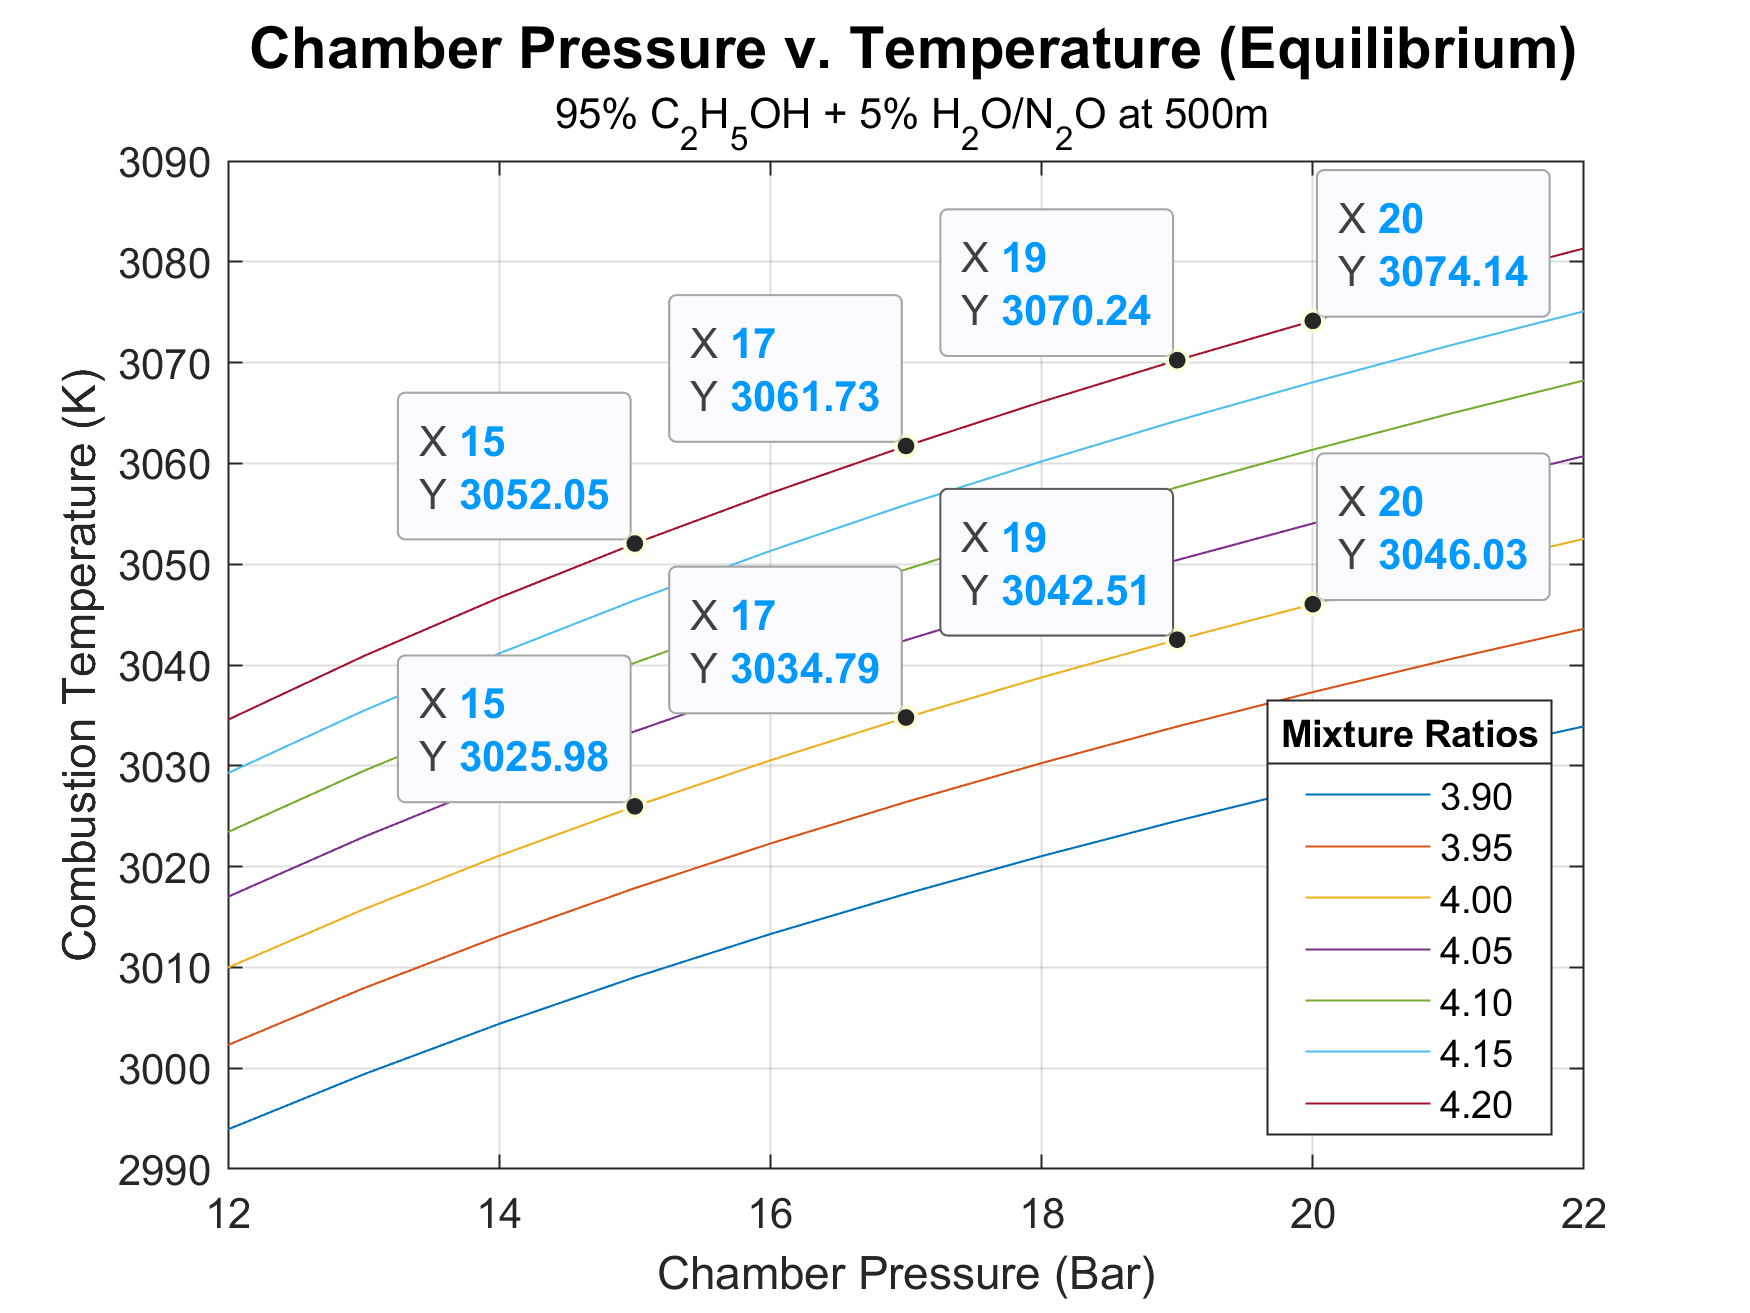
\includegraphics[scale=0.5, width=0.9\textwidth]{cp_temp_mix_labeled} % second figure itself
        \caption{Combustion temperature vs chamber pressure and numerous mixture ratios.}
        \label{fig:cp_temp}
    \end{minipage}
\end{figure} 
\begin{figure}
    \centering
    \begin{minipage}{0.475\textwidth}
        \centering
        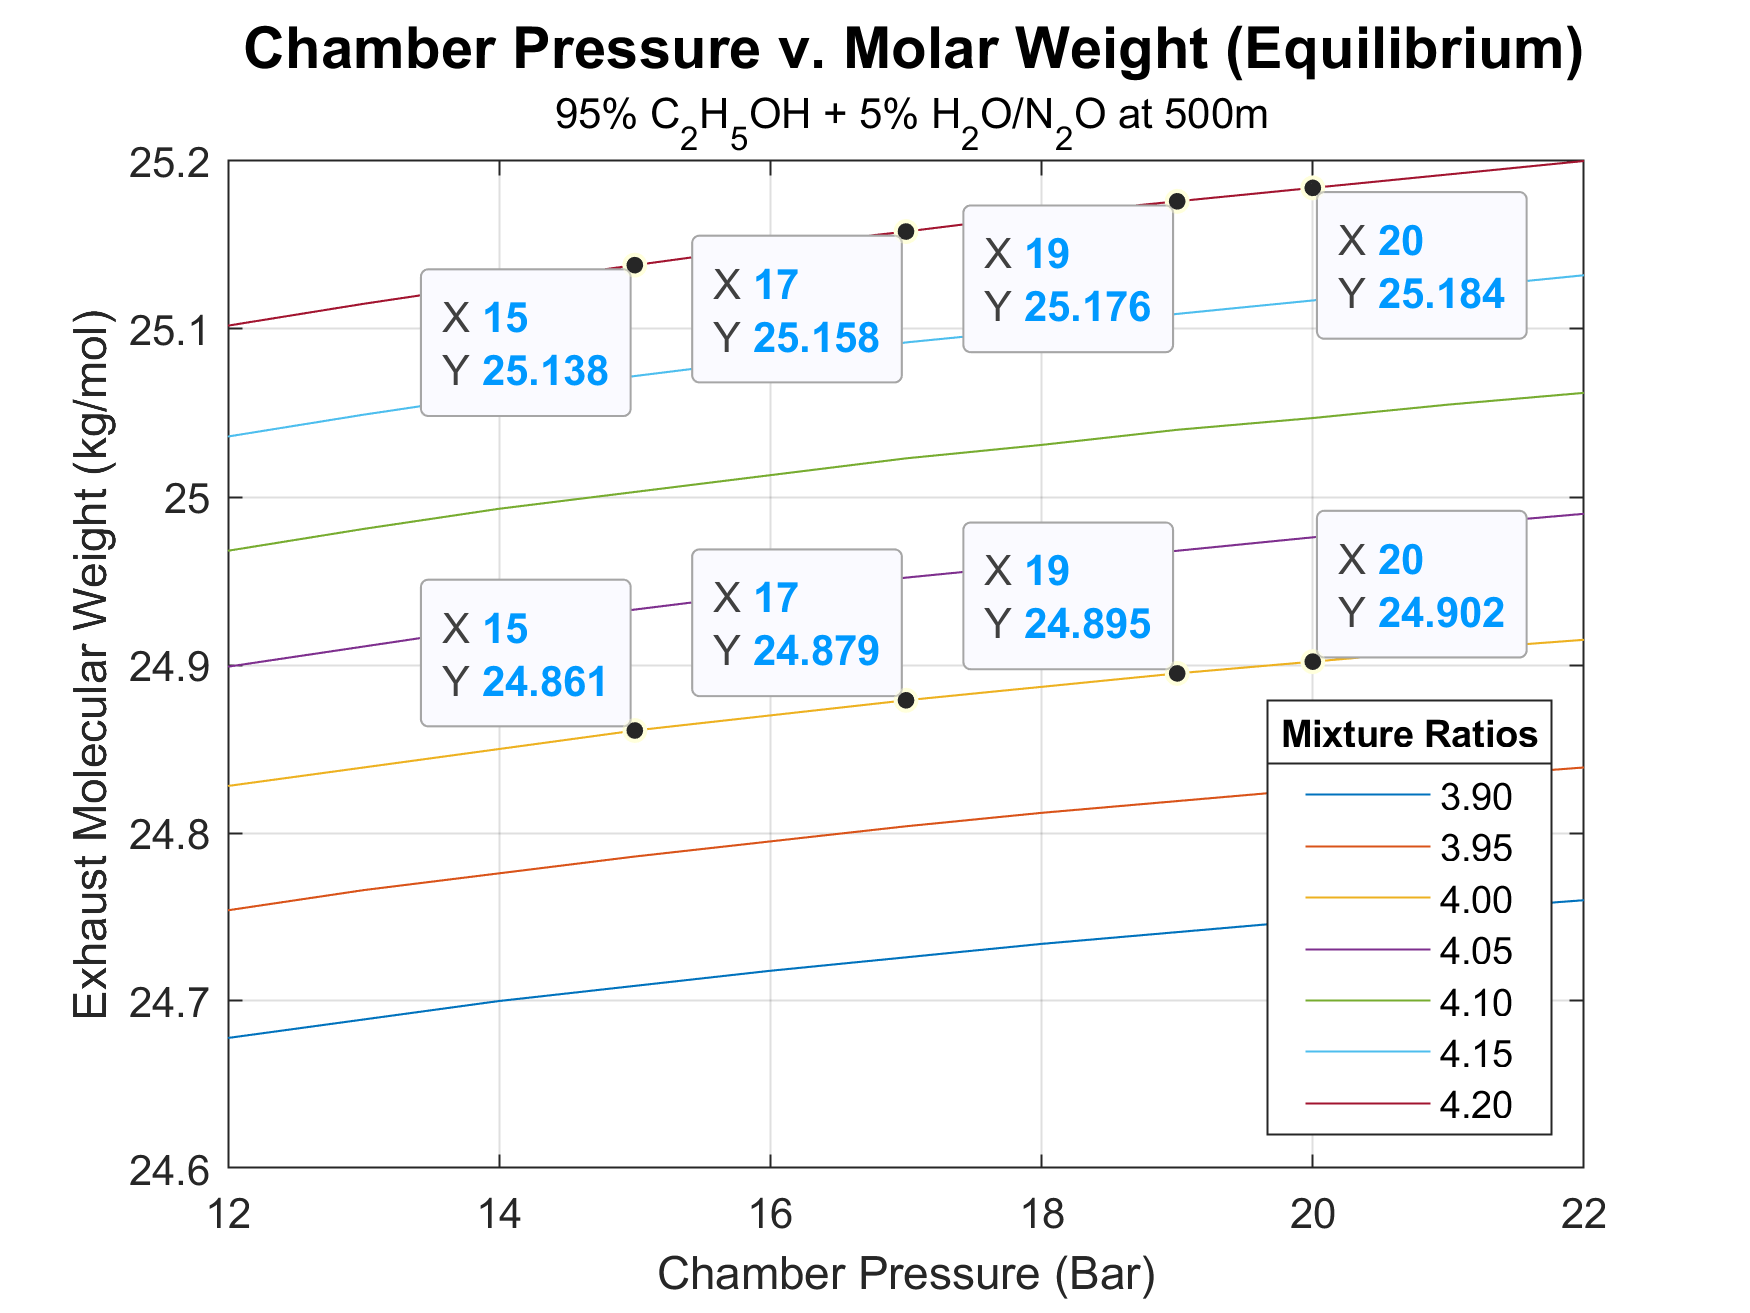
\includegraphics[scale=0.5, width=0.9\textwidth]{cp_molar_mix_labeled} % first figure itself
        \caption{Gas molecular mass vs chamber pressure and numerous mixture ratios.}
        \label{fig:cp_molar}
    \end{minipage}\hfill
    \begin{minipage}{0.475\textwidth}
        \centering
        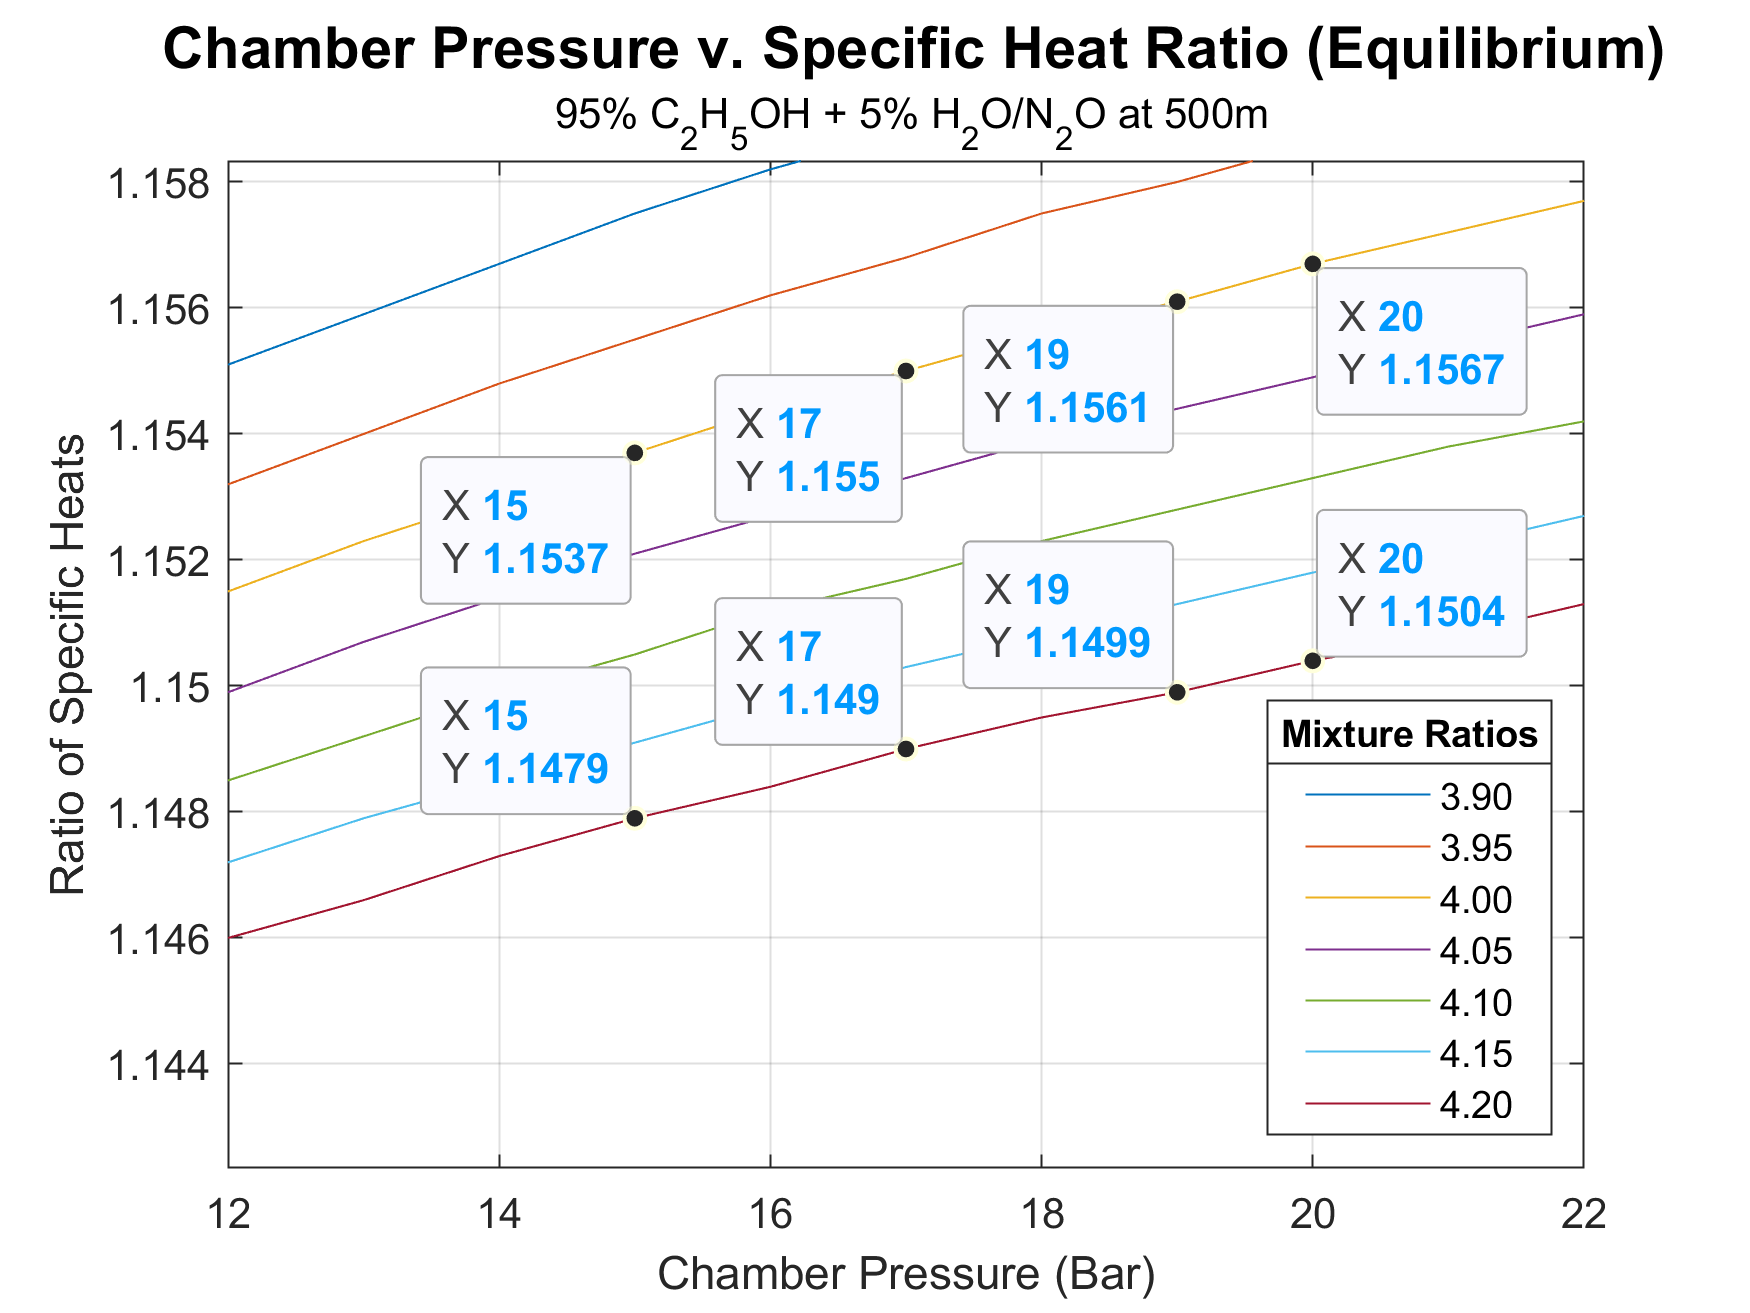
\includegraphics[scale=0.5, width=0.9\textwidth]{cp_gamma_mix_labeled} % second figure itself
        \caption{Ratio of specific heats vs chamber pressure and numerous mixture ratios.}
        \label{fig:cp_gamma}
    \end{minipage}
\end{figure}

\subsection{Chamber Pressure and Mixture Ratio Selection}
\hspace{\parindent} The first step is to realize the theoretical maximum performance to be expected from our propellant combination.  95\% ethyl alcohol (ethanol) was chosen for its availability, low pricing, and a modest specific impulse. A 95\% dilution (by mass) with water was chosen as to lower the expected combustion chamber temperature. This trade-off sacrifices some $I_{sp}$ but reduces engineering complexity as regenerative and film cooling circuits may not be required. Industrial nitrous oxide was chosen as the main oxidizer for its self-pressurizing characteristics, non-cryogenic nature as opposed to liquid oxygen, relative ease to obtain, and a modest $I_{sp}$ with ethanol.
Using CEA, an open-source thermodynamics library provided by NASA's Glenn Research Center, critical data describing propellant combustion characteristics could be obtained. Numerical Python scripts were written to iterate through various combustion chamber pressures and mixture ratios and interface with CEA, and MATLAB scripts were used to parse and graph the CEA outputs as shown in Figures \ref{fig:cp_cstar}, \ref{fig:cp_temp}, \ref{fig:cp_molar}, and \ref{fig:cp_gamma}. Mixture ratios of 4.0 and 4.2 are labeled at certain chamber pressures. All dependent-variable properties (characteristic velocity $C^{*}$, combustion temperature $T_{c}$, exhaust molar mass $M$, and exhaust specific heat ratio $\gamma$) were permuted assuming shifting equilibrium flow and at an operational altitude of 500 m. 

A mixture ratio of 4.0 was chosen for Aphlex 1B mainly in the interest of a conservative combustion temperature of around 3026 K and a middle-of-the-line theoretical $C^{*}$ of around 1570 m/s, given a chamber pressure of 15 bar. This chamber pressure was chosen to minimize upstream fluid pressures and thus tank weight requirements, while also considering two additional design constraints that were not mentioned above but are nevertheless valid guiding parameters: a fluid flow velocity of less than 6 m/s to avoid water hammer effects [Zucrow Laboratories] and a pressure drop across the injector of around 25\% of the designated chamber pressure [Michigan Aeronautical Science Association]. The former of these additional guidelines is to avoid feed-coupled combustion instabilities that may be observed when the $\delta p$ across the injector is not adequately high. These guidelines further encourage a lower chamber pressure, and thus a conservative value of 15 Bar was chosen.

\section{Propulsion System Design}
\hspace{\parindent} The following section outlines the design process for Aphlex 1B, our second-generation bi-propellant liquid rocket engine, set to fly on our 30 kg launch vehicle, Callisto 1, given the objectives and data obtained in the previous section.

\subsection{Nozzle Design}

\begin{table}[!htb]
\centering
\begin{tabular}{ |p{5cm}||p{4cm}|p{1cm}|p{2cm}|  }
\hline
\multicolumn{4}{|c|}{Design Parameters} \\
\hline
Name & Value & Unit & Uncertainty \\
\hline
Propellant (Fuel)  &  Ethanol ($C_{2}H_{5}OH$, $95\%$)   &  N/A  &  N/A \\
Propellant (Oxidizer)  &  Nitrous oxide ($N_{2}O$) & N/A  &  N/A \\
$O/F$, Oxidizer/fuel ratio &  4.0  &  $N/A$  &   $\pm 1 \%$ \\
$F_{t}$, Nominal thrust &  1.50 &  $kN$  &  $\pm 0.1 \%$ \\
$P_{c}$, Chamber static pressure &  $1.5 \times 10^{6}$  &  $Pa$  &  $\pm 0.1 \%$ \\
$P_{e}$, Ambient pressure &  $9.5540 \times 10^{4}$  &  $Pa$  &  $\pm 0.1 \%$ \\
$T_{c}$, Chamber static temperature &  3025.98  &  $K$  &  $\pm 0.01 \%$  \\
$M$, Exhaust molecular mass &  24.861  &  $kg/mol$  &   $\pm 0.01 \%$ \\
$\gamma$, Specific heat ratio  &  1.1537  &  $N/A$  &   $\pm 0.001 \%$ \\
\hline
\end{tabular}
\caption{Summary of exhaust gas properties and fluid parameters.}
\label{table:gas_parameters}
\end{table}

\begin{equation} \label{eq:ambient_temperature}
T_{3} = 15.04 - 0.00649 h 
\end{equation}
\begin{equation} \label{eq:ambient_pressure}
P_{3} = \left[101.29 \times \left( \frac{T + 273.1}{288.08} \right) ^ {5.256} \right] \times 1000
\end{equation}

The nozzle design process followed standard procedures outlined in Rocket Propulsion Elements \cite{rpe} and open-source NASA documents. The thermodynamic properties of the exhaust gas and other important parameters are summarized and compiled in Table \ref{table:gas_parameters}. The ambient pressure was calculated using NASA Glenn Research Center's Earth Atmosphere Model for an altitude within the troposphere (less than 11000 meters), as shown in Equations \ref{eq:ambient_temperature} and \ref{eq:ambient_pressure}, where $T_{3}$ represents the ambient temperature in Kelvin, $h$ is the altitude in meters, $P_{3}$ is the ambient pressure in Pascals.

Assuming fully isentropic flow (by definition both adiabatic and reversible) in the supersonic nozzle with choked flow conditions at the throat, an ideal converging-diverging (de Laval) nozzle can be characterized. The first parameter to calculate is the controlling area ratio
\begin{equation} \label{eq:area_ratio}
\frac{A_{t}}{A_{2}} = \left( \frac{\gamma + 1}{2} \right) ^{1/(\gamma - 1)} \left( \frac{p_{2}}{p_{1}} \right) ^{1/\gamma} \sqrt{ \frac{\gamma + 1}{\gamma - 1} \left[ 1 - \left( \frac{p_{2}}{p_{1}} \right) ^{(\gamma - 1)/\gamma} \right] }
\end{equation}
where $A_{t}$ is the cross-sectional area of the throat, $A_{2}$ is the cross-sectional area at nozzle exit, and $p_{1}$ and $p_{2}$ are the chamber pressure and exit pressure respectively. Equation \ref{eq:area_ratio} is also often referred to as the inverse of the expansion ratio $\epsilon$, since $\epsilon = A_{2}/A_{t}$. Evaluating Equation \ref{eq:area_ratio} gives
\begin{equation*} 
\frac{A_{t}}{A_{2}} = \left( \frac{2.15}{2} \right) ^{1/0.15} \left( \frac{9.6 \times 10^{4}}{1.5 \times 10^{6}} \right) ^{1/1.15} \sqrt{ \frac{2.15}{0.15} \left[ 1 - \left( \frac{9.6 \times 10^{4}}{1.5 \times 10^{6}} \right) ^{0.15/1.15} \right] } = 0.307
\end{equation*}
Notice the substitution of $p_{2}$ for $P_{e}$ as specified in Table \ref{table:gas_parameters}, since in an ideal nozzle, the exhaust gas should expand to ambient pressure. The expansion ratio $\epsilon$ is simply
\begin{equation*}
\epsilon = A_{2}/A_{t} = 1/AR = 1/0.307 = 3.26
\end{equation*}
Next, we can find the ideal exit velocity $v_{2}$, sometimes denoted as $c$:
\begin{equation} \label{eq:exit_velocity}
v_{2} = \sqrt{ \frac{2\gamma}{\gamma - 1} \left( \frac{R_{u}T_{1}}{M} \right) \left[ 1- \left( \frac{p_{2}}{p_{1}} \right) ^{(\gamma - 1)/\gamma} \right] }
\end{equation}
where $R_{u}$ is the universal gas constant of 8314.3 J/kg mol-K and $M$ is the molecular mass of the gas as shown in Table \ref{table:gas_parameters}. Evaluating gives
\begin{equation*} 
v_{2} = \sqrt{ \frac{2 * 1.15}{0.15} \left( \frac{8314.3 * 3026}{24.86} \right) \left[ 1- \left( \frac{9.6 \times 10^{4}}{1.5 \times 10^{6}} \right) ^{0.15/1.15} \right] } = 2162.3 \; m/s
\end{equation*}
Next, the mass flow rate $\dot{m}$ can be calculated explicitly noting that $v_{2} = c$, since earlier it was stated that $p_{2} = p_{3}$:
\begin{equation} \label{eq:mdot}
\dot{m} = F_{t}/c = 1500/2162.3 = 0.694 \; kg/s
\end{equation}
Solving using our chosen $O/F$ ratio of 4.0 for each independent propellant $\dot{m}$ gives
\begin{align*} 
\dot{m}_{o} = \dot{m} * (4/5) = 0.694 * (4/5) = 0.555 \; kg/s \\
\dot{m}_{f} = \dot{m} * (1/5) = 0.694 * (1/5) = 0.139 \; kg/s
\end{align*}
Next, we arrive at the throat area:
\begin{equation} \label{eq:throat_area}
A_{t} = \frac{\dot{m}}{p_{1}} \sqrt{ \frac{(R_{u}/M)T_{1}}{\gamma [2/(\gamma + 1)]^{(\gamma + 1)/(\gamma - 1)}} }
\end{equation}
Evaluating Equation \ref{eq:throat_area} gives
\begin{equation*} 
A_{t} = \frac{0.694}{1.5 \times 10^{6}} \sqrt{ \frac{(8314.3/24.86) * 3026}{1.15 [2/(2.15)]^{(2.15)/(0.15)}} } = 7.29 \times 10^{-4} \; m^{2} = 7.29 \; cm^{2}
\end{equation*}
Using this calculated throat area and the expansion ratio, the exit area is simply
\begin{equation} \label{eq:exit_area}
A_{2} = \epsilon * A_{t} = 3.26 * 7.29 \times 10 ^{-4} = 2.38 \times 10^{-3} \; m^{2} = 23.8 \; cm^{2}
\end{equation}
From the parameters calculated thus far, we can calculate some useful performance metrics such as $I_{sp}$ and thrust coefficient $C_{F}$:
\begin{equation} \label{eq:specific_impulse}
(I_{sp})_{opt} = F_{t}/(\dot{m} * g_{0}) = c/g_{0} = 2162.3/9.81 = 220.42 \; sec
\end{equation}
where $g_{0}$ is the acceleration due to gravity at Earth's surface. $C_{F}$ is
\begin{equation} \label{eq:thrust_coefficient}
(C_{F})_{opt} = \frac{F_{t}}{p_{1}A_{t}} = \frac{1500}{1.5 \times 10^{6} * 7.29 \times 10 ^{4}} = 1.372
\end{equation}
Note that under a more rigorous derivation, $C_{F}$ can be seen to be a key parameter for analysis and varies depending on $\gamma$, the nozzle expansion ratio $\epsilon$, and the pressure ratio $p_{1}/p_{2}$. Normally, $C_{F}$ is experimentally determined by measuring chamber pressure, throat diameter, and thrust. The optimal $C_{F}$ and therefore $F_{t}$ occur when $p_{2} = p_{3}$.

Finally, the physical dimensions of the nozzle can be determined using simple trigonometry via a standard convergence half-angle $\alpha$ of $\ang{45}$ and a standard divergence half-angle $\beta$ of $\ang{15}$. The characteristic chamber length $L^{*}$, a parameter used for characterizing the necessary chamber volume for adequate mixing and combustion of the propellants, must be more carefully considered. Ideally, $L^{*}$ is purely a function of the chemistry of the propellant combination and is often based upon previous successful engine designs \cite{rpe}. However, due to the dynamical and complex nature of nitrous oxide, such as exothermic decomposition after vaporization in the injector and a high density sensitivity to temperature, a more sophisticated model is needed to calculate $L^{*}$. Palacz proposes an explicit equation for finding the ideal $L^{*}$ for a nitrous oxide system, and empirically determined an ideal range for an $NO_{x}$/ethanol system of $L^{*}$ values from 125.6 cm to 167.8 cm \cite{nitrous-paper}. This range is confirmed by Sutton and Biblarz, as $L^{*}$ values of between 1.0 m and 1.5 m are expected with ethanol systems. A low-range $L^{*}$ value of 1.25 m was chosen as a smaller form factor is desired over perfect combustion efficiency. $L^{*}$ is mathematically defined as
\begin{equation} \label{eq:l_star}
L^{*} = \frac{V_{c}}{A_{t}} = \frac{\pi r_{c}^{2} L{c}}{A_{t}} \; \Longrightarrow \; L_{c} = \frac{A_{t} L^{*}}{\pi r_{c}^{2}}
\end{equation}
where $L_{c}$ is the length of the chamber and $r_{c}$ is the radius of the chamber. It is apparent that the a desired form factor can be obtained by adjusting either the radius or the length of the chamber. Through iteration, a chamber radius $r_{c}$ of 4.0 cm was chosen. The only constraint on the chamber radius is the contraction ratio, defined as $A_{1}/A_{t}$ (the ratio of chamber area to throat area), which must achieve a value of 4.0 or more \cite{rpe}. A trivial area calculation can be performed to confirm that this constraint is satisfied: $CR =  \pi r_{c}^{2}/A_{t} = 5.03 \times 10^{-4} \; m^{2} / 7.29 \times 10^{-4} \; m^{2} = 6.90 > 4.0$. The chamber length is therefore
\begin{equation*}
L_{c} = \frac{A_{t} L^{*}}{\pi r_{c}^{2}} = \frac{(7.29 \times 10^{-4} \; m^{2})(1.25 \; m)}{5.03 \times 10^{-4} \; m^{2}} = 0.1813 \; m = 18.13 \; cm
\end{equation*}

\begin{table}[!htb]
\centering
\begin{tabular}{ |p{6cm}||p{2cm}|p{1cm}| }
\hline
\multicolumn{3}{|c|}{Calculated Performance Parameters} \\
\hline
Name & Value & Unit \\ 
\hline
$\dot{m}$, Total mass flow rate  &  0.694  &  $kg/s$  \\
$\dot{m}_{f}$, Fuel mass flow rate &  0.555  &  $kg/s$  \\
$\dot{m}_{o}$, Oxidizer mass flow rate &  0.139  &  $kg/s$  \\
$v_{2}$, Exhaust velocity & 2162.3 & $m/s$ \\
$(I_{sp})_{opt}$, Specific impulse (optimal) & 220.42 & $s$ \\
$(C_{F})_{opt}$, Thrust coefficient (optimal) & 1.372 & $N/A$ \\
\hline
\end{tabular}
\caption{Summary of engine performance parameters.}
\label{table:calculated_parameters}
\end{table}

\begin{table}[!htb]
\centering
\begin{tabular}{ |p{6cm}||p{2cm}|p{1cm}| }
\hline
\multicolumn{3}{|c|}{Calculated Dimensional Parameters} \\
\hline
Name & Value & Unit \\ 
\hline
$\alpha$, Convergence half-angle &  45  &  $deg$ \\
$\beta$, Divergence half-angle &  15  &  $deg$  \\
$A_{t}$, Throat area  & $7.29 \times 10^{-4}$ & $m^{2}$ \\
$A_{2}$, Exit area & $2.38 \times 10^{-3}$ & $m^{2}$ \\
$A_{c}$, Chamber cross-sectional area & $5.03 \times 10^{-4}$ & $m^{2}$ \\
$R_{t}$, Throat radius & $15.23$ & $mm$ \\
$R_{2}$, Exit radius & $27.52$ & $mm$ \\
$R_{c}$, Chamber radius & $40.0$ & $mm$ \\
$L_{c}$, Chamber length & $181.3$ & $mm$ \\
$\epsilon$, Expansion ratio  &  3.26  &  $N/A$  \\
$CR$, Contraction ratio  &  6.9  &  $N/A$  \\
\hline
\end{tabular}
\caption{Summary of physical nozzle dimensions.}
\label{table:calculated_dimensions}
\end{table}

\begin{figure}
\centering
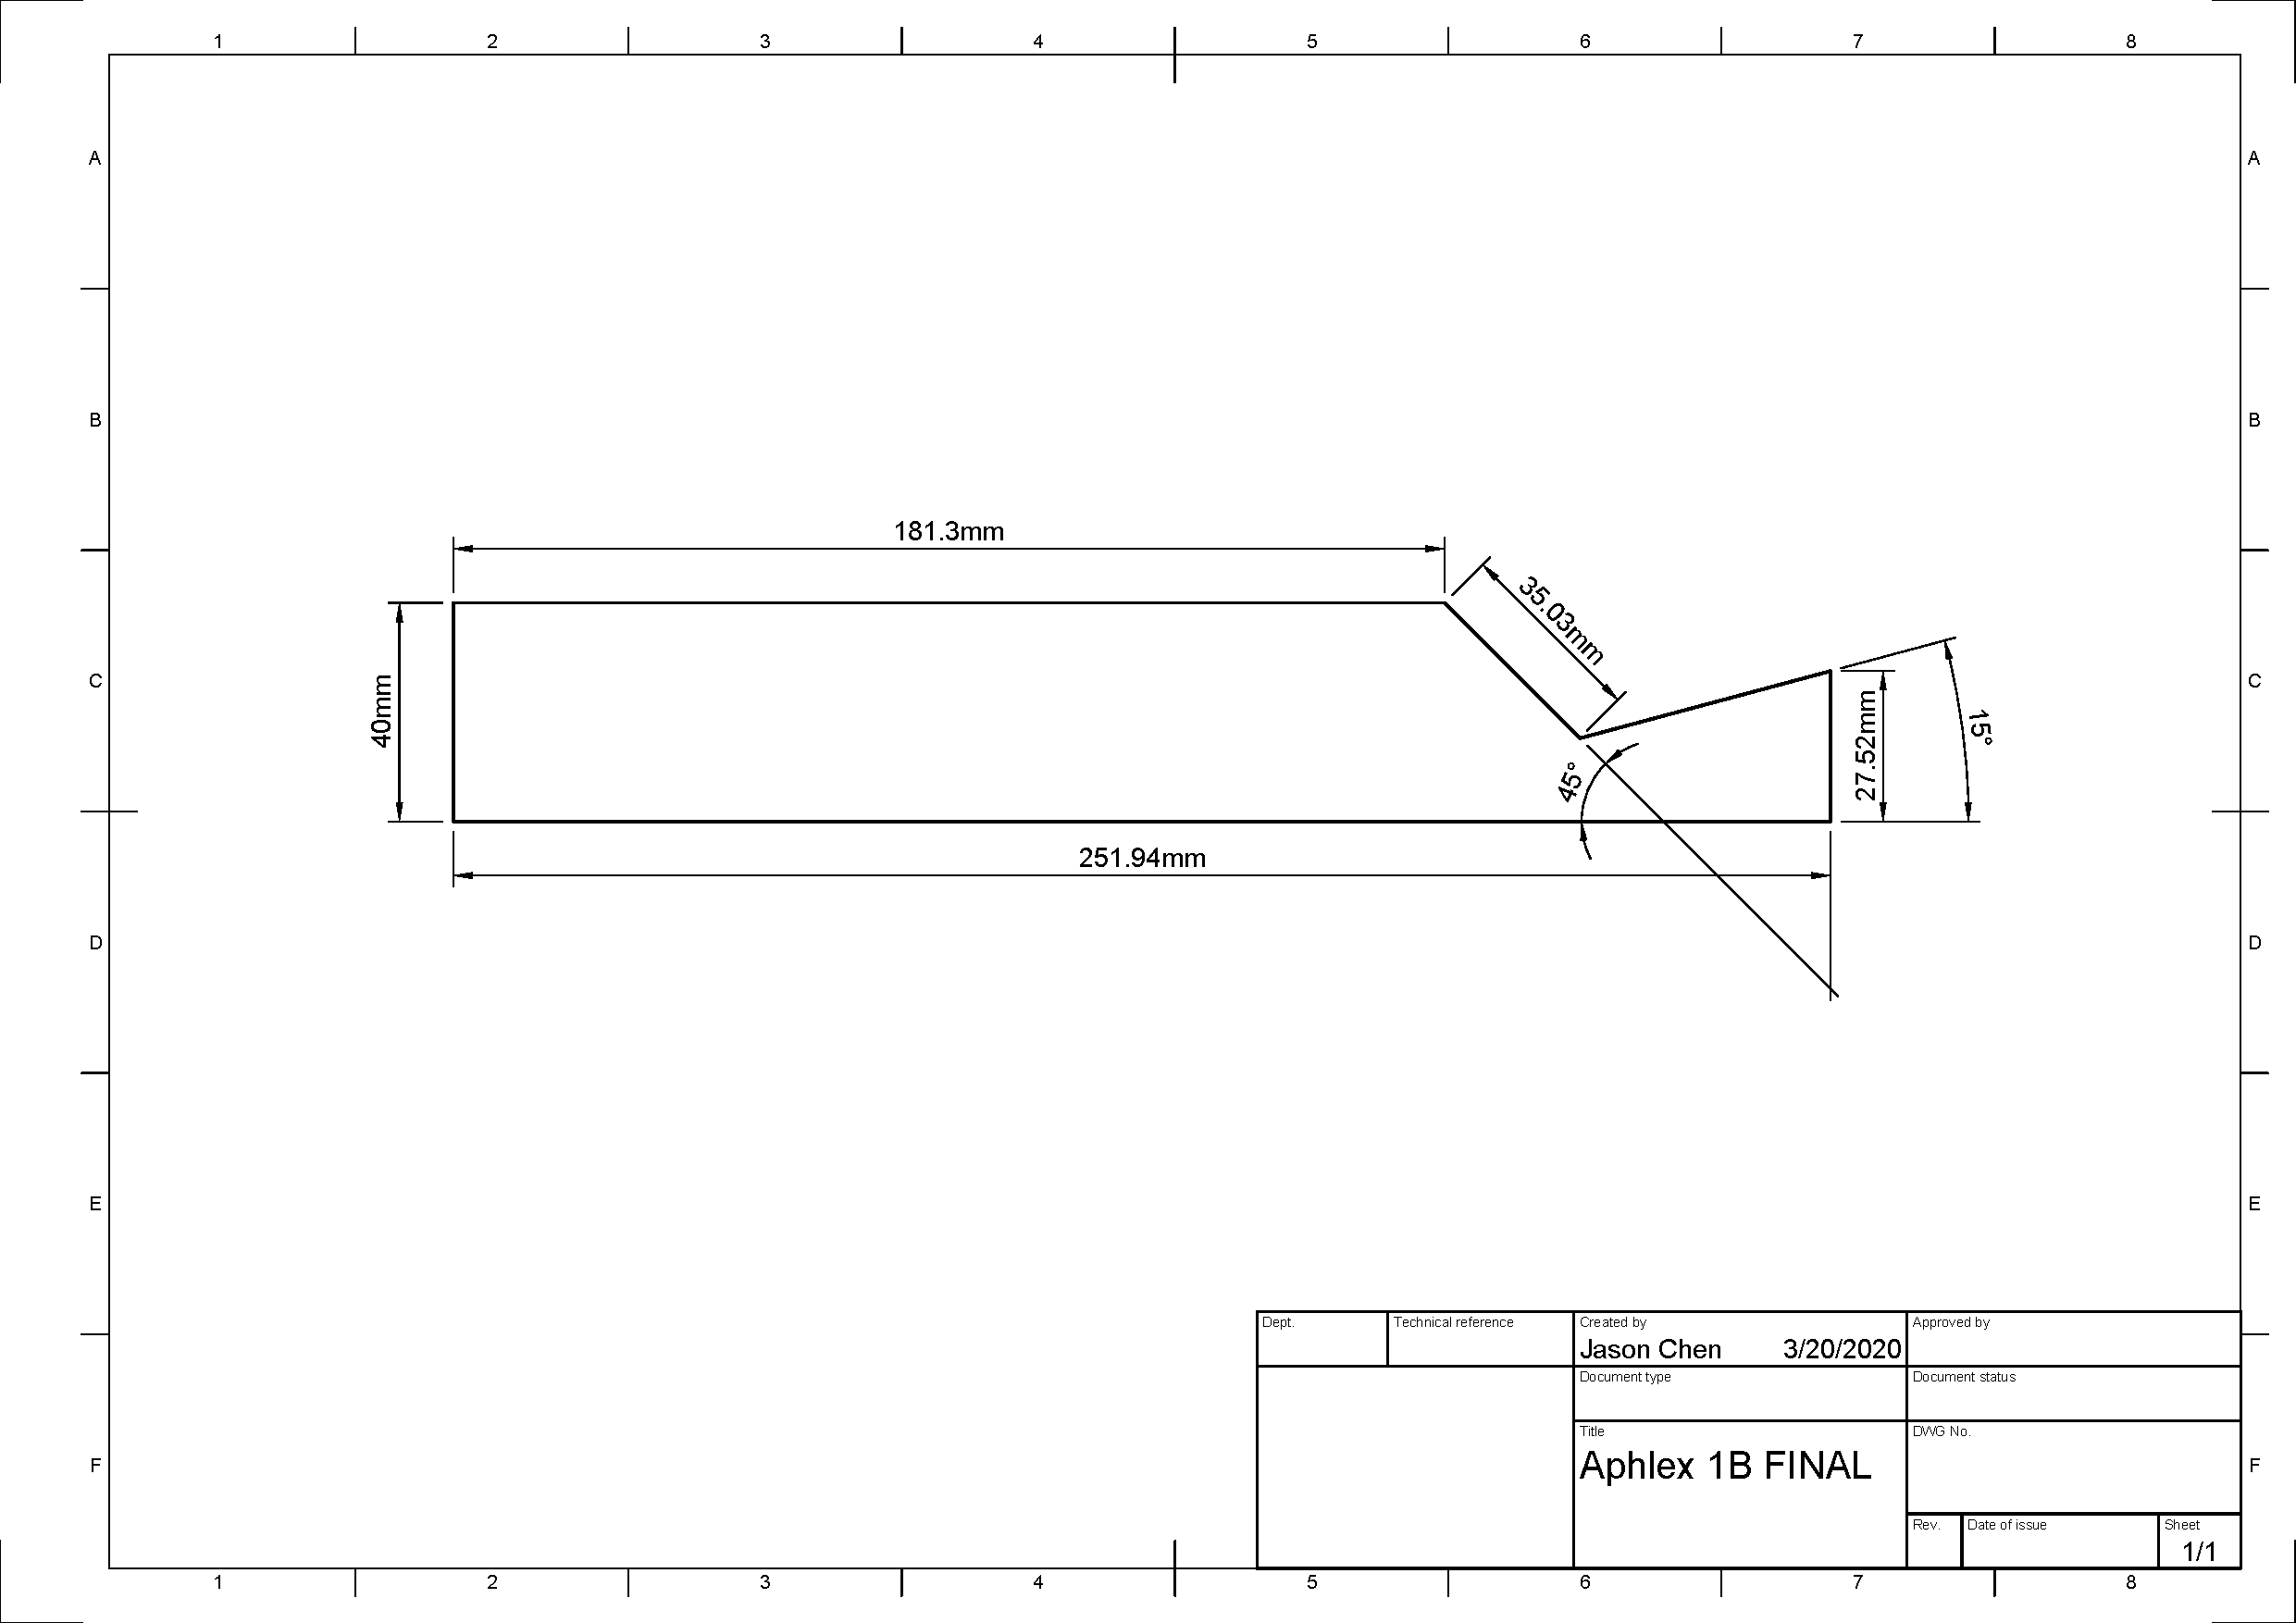
\includegraphics[scale=0.5, width=0.9\textwidth, trim={6.5cm 12.5cm 5.5cm 9cm}, clip]{aphlex1b-drawing} % Trim order is left, bottom, right, top
\caption{Aphlex 1B drawing with a conical nozzle and given dimensions.}
\label{fig:conical_nozzle_drawing}
\end{figure}

Table \ref{table:calculated_parameters} shows the calculated engine parameters and Table \ref{table:calculated_dimensions} shows the calculated physical nozzle dimensions. Using the data from Table \ref{table:calculated_dimensions}, a basic conical nozzle can be realized.

Figure \ref{fig:conical_nozzle_drawing} shows the basic conical nozzle for Aphlex 1B created using the given dimensions. Although a conical nozzle may exhibit an advantage in its ease of manufacturing, it is sub-optimal for performance since 1) the exhaust is not exiting the nozzle completely parallel to the nozzle axis, which results in lateral losses of energy, 2) the sharp convex corner at the throat generates shocks which are not adequately dissipated by a conical nozzle, and 3) the small divergence half-angle ensures a long diverging section, which increases engine mass. To address these issues, most modern nozzles are so-called ``bell'' nozzles, whose diverging section includes a straightening section to address the first issue and inherently addresses the third issue by having a more rapidly expanding cross-section as compared to conical nozzles. To neutralize the Prandtl-Meyer expansion fans generated at the sharp corner of the throat, a numerical technique called the Method of Characteristics (MOC) is used to generate the nozzle contour. 

\begin{figure}
\centering
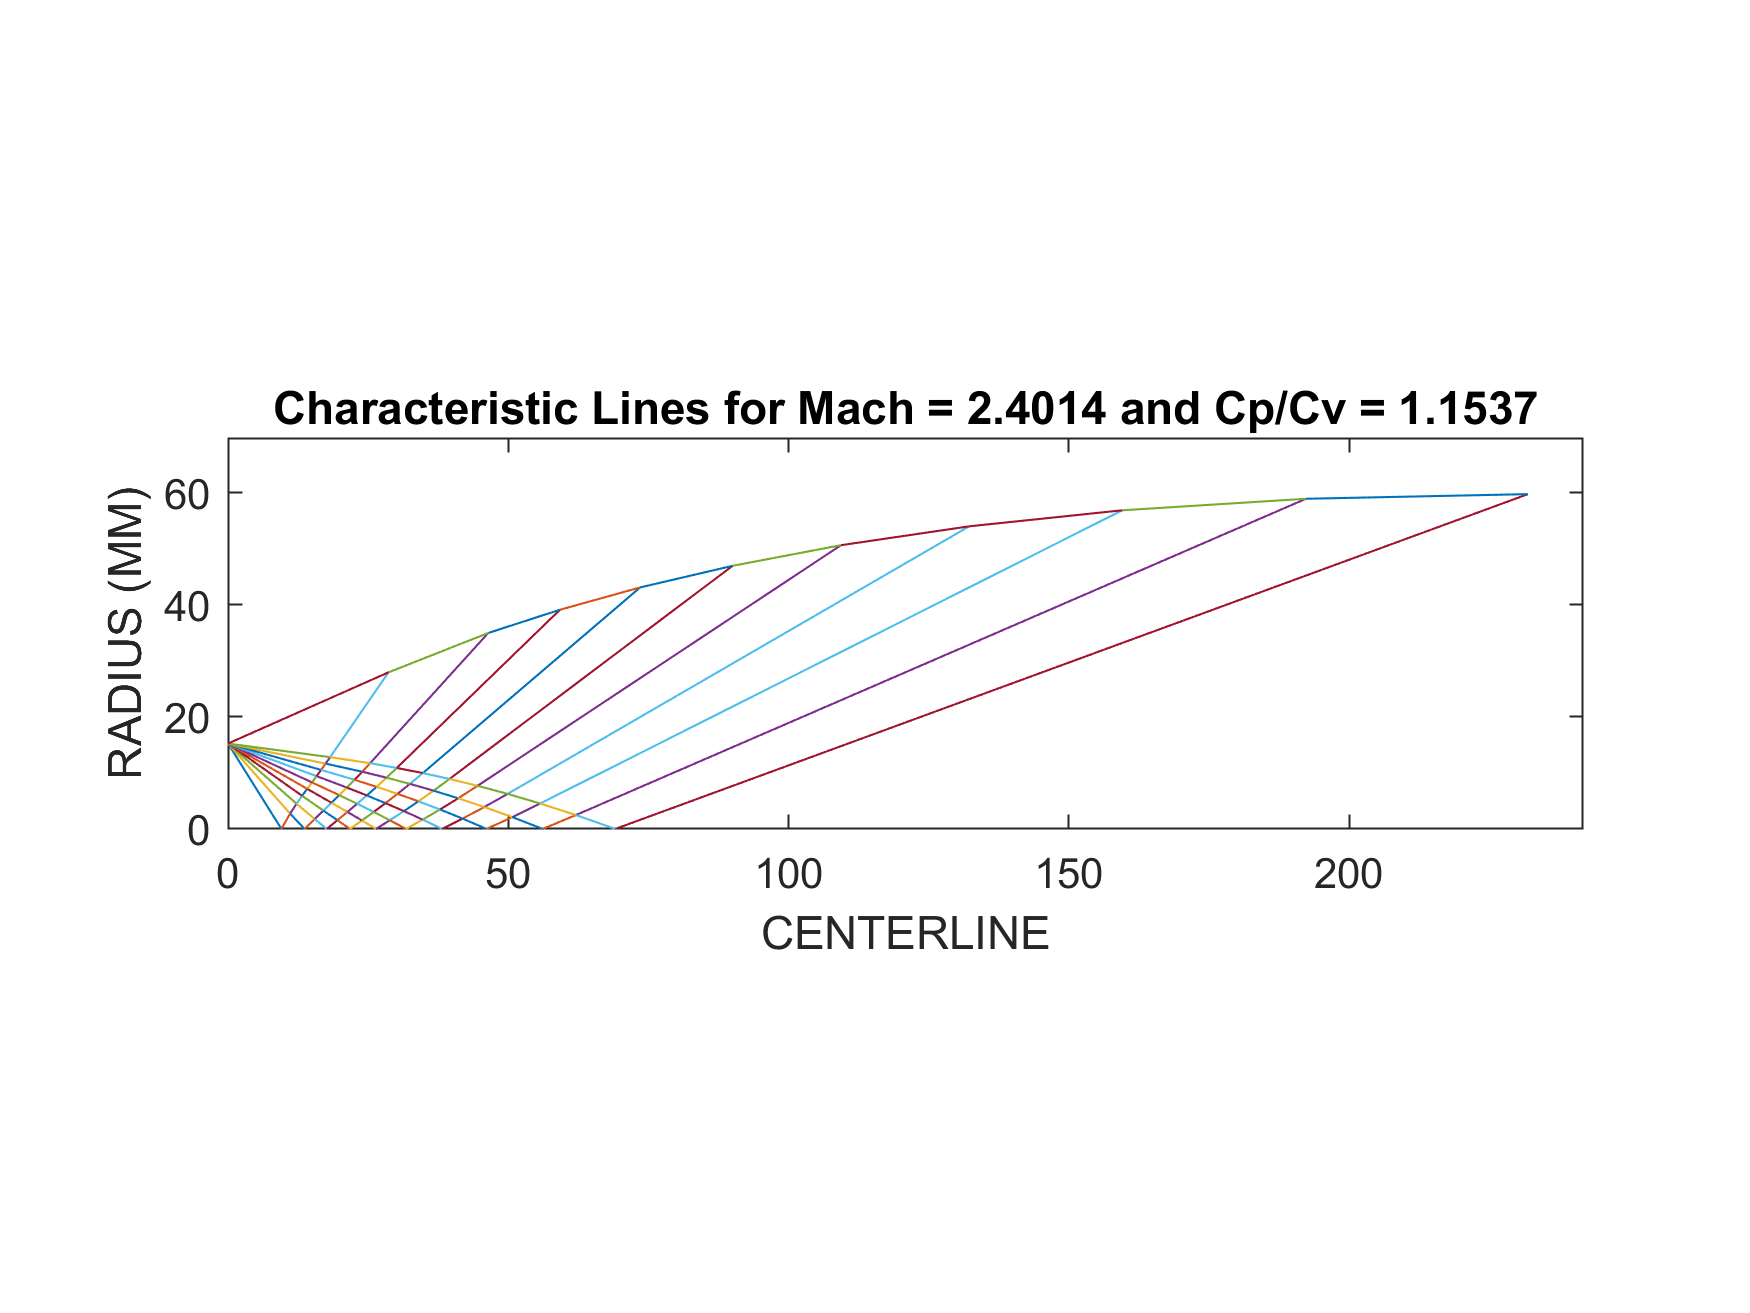
\includegraphics[scale=0.5, width=0.9\textwidth, trim={0.5cm 2.5cm 0.5cm 3.25cm}, clip]{moc} % Trim order is left, bottom, right, top
\caption{MATLAB visualization for MOC. Shown are the characteristic lines and the generated nozzle contour.}
\label{fig:moc}
\end{figure}

In brief, MOC propagates characteristic lines emanating from the throat, and by using equations to model characteristic interactions and reflections, it is able to generate a nozzle contour to precisely neutralize (reflect in a manner parallel to the nozzle axis) these expansion fans. A MATLAB script was written to execute and create the MOC nozzle, which can be found on our Project Caelus propulsion GitHub repository at \url{https://github.com/ProjectCaelus/propulsion/blob/master/nozzle-calculations/moc_nozzle.m}. Its output is shown in Figure \ref{fig:moc}. The Cartesian points representing the generated wall contour were exported as a CSV file, which was then imported into our computer-aided design (CAD) program, Fusion 360, where a best-fit nth-order spline was used to finalize the diverging contour. Although the shape of the diverging section can be optimized significantly, the precise shape of the nozzle converging section has not been found to heavily impact engine performance and is therefore smoothed under the guidelines of Dr. GVR Rao's parabolic approximation method \cite{rpe}\cite{rao}. 

\begin{figure}
\centering
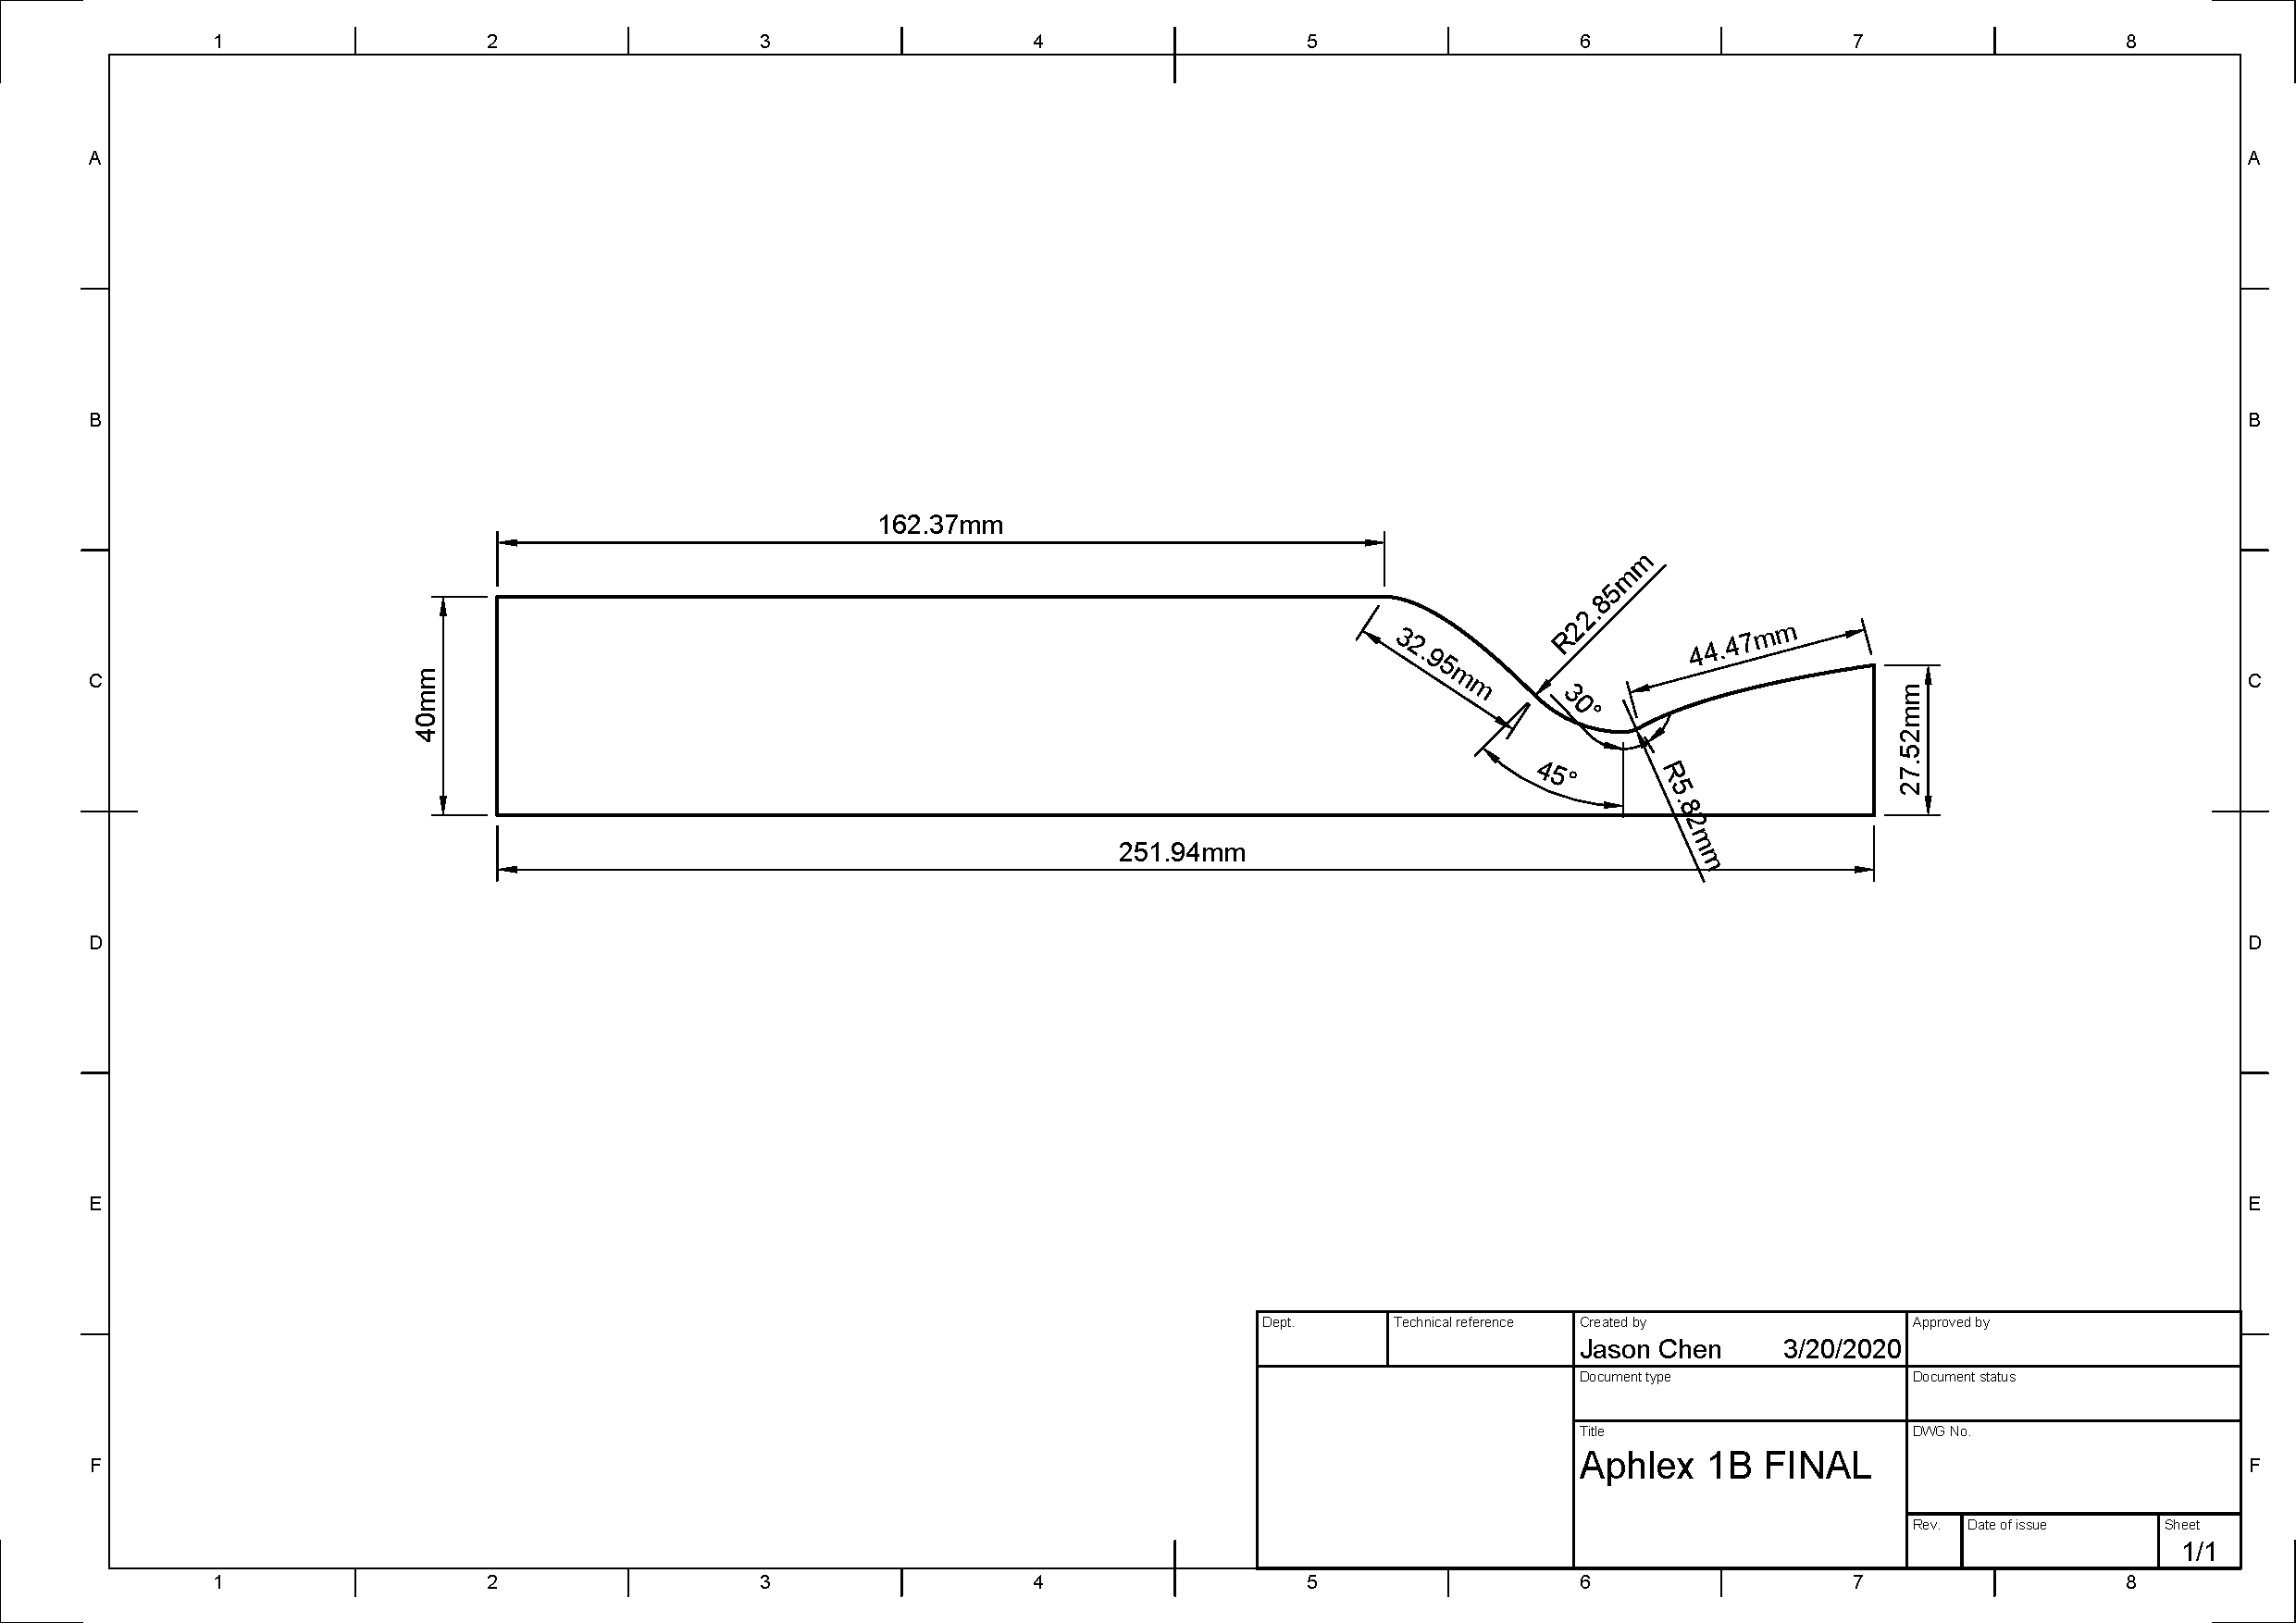
\includegraphics[scale=0.5, width=0.9\textwidth, trim={7.25cm 12.5cm 5.5cm 9cm}, clip]{aphlex1b-drawing-2} % Trim order is left, bottom, right, top
\caption{Aphlex 1B drawing with a MOC nozzle and given dimensions.}
\label{fig:moc_nozzle_drawing}
\end{figure}

\subsection{Injector Design}

\hspace{\parindent} The injector serves two main purposes in a liquid rocket engine: the adequate mixing (atomization) of the incoming propellant streams to ensure maximum combustion efficiency and the prevention or minimization of combustion instabilities. Some injectors additionally implement film cooling to aid in reducing the thermal load of the chamber and nozzle walls, however, our system relies solely on the heat capacity of the chamber walls and a thin ablative layer to maintain wall integrity. This is done since it would save propellant mass that would otherwise be wasted for film cooling and due to the relatively short burn time of our system. 

\subsubsection{Selection of Element Type}

There are many types of injector elements, each with unique advantages and disadvantages. The injector types considered were the triplet (fuel-centered) unlike impinging injector and the like-on-like doublet impinging injector, due to 1) our limited manufacturing capabilities 2) a fairly unbalanced O/F ratio 3) both types exhibiting good mixing and atomization properties and 4) the abundance of historical experience and data with both injector types. Both the coaxial swirl and pintle types were deemed either too complex to manufacture or too difficult to characterize due to a limited amount of available documentation. NASA's SP-8089 conference document on liquid engine injector design suggests that the best way to characterize both the individual orifice geometries and the overall injector geometry for unlike impinging injectors is through diameter ratios. Vigorous cold flow and other empirically testing methods at the time were used and have found correlations between the driving orifice diameter ratio with the optimum mixing efficiency. The correlation found was
\begin{equation} \label{eq: diameter_ratio}
    \left( \frac{d_{c}}{d_{ou}} \right)^{2} = M \left[ \frac{\rho_{ou}}{\rho_{c}} \left( \frac{\dot{m}_{c}}{\dot{m}_{ou}} \right)^{2} \right]^{0.7}
\end{equation}
where $d_{c}$ is the diameter of center orifice, $d_{ou}$ is the diameter of an outside individual orifice, M is an experimentally-determined mixing factor coefficient, $\rho$ represents liquid density, and $\dot{c}$ and $\dot{m}_{ou}$ are the center mass flow rate and outside mass flow rate respectively. It is cited that for a 2-on-1 element type, M has a value of 1.6. Using Equation \ref{eq: diameter_ratio}, we find that our controlling diameter ratio is
\begin{equation*}
    \frac{d_{c}}{d_{ou}} = \sqrt{M \left[ \frac{\rho_{ou}}{\rho_{c}} \left( \frac{\dot{m}_{c}}{\dot{m}_{ou}} \right)^{2} \right]^{0.7}} = \sqrt{1.6 \left[ \frac{772.25 \; kg/m^{3}}{789 \; kg/m^{3}} \left( \frac{0.1389 \; kg/s}{0.5556 \; kg/s} \right)^{2} \right]^{0.7}} = 0.4757
\end{equation*}
Since this diameter ratio is not reasonably near 1.22 (as suggested by NASA SP-8089), we can assume this correlation would not be accurate and that there will be potentially drastic losses in mixing efficiency. Thus, this suggests that a like-on-like system is required. 

\subsubsection{Main Injector Parameterization}

Since like-on-like elements will have a 1 to 1 diameter and momentum ratio, we can begin determining the pressure drop and mass flow rate through each individual orifice. Rocket Propulsion Elements (RPE) provides and equation for the volumetric flow rate $Q$ (and therefore $\dot{m}$ since $\rho$ is constant) as shown below:
\begin{equation} \label{eq: discharge}
    \dot{m} = Q \rho = C_{d} A \sqrt{2 \rho \Delta p} \; \Longrightarrow \;
    \Delta p = \left[ \left( \frac{\dot{m}}{C_{d} A} \right)^{2} \right] / 2 \rho
\end{equation}
where $C_{d}$ is a dimensionless discharge coefficient that is experimentally determined and a function of the orifice geometry, $A$ is the area of the orifice, and $\Delta p$ is the pressure drop across the orifice. Flow velocity is similar:
\begin{equation} \label{eq: flow_velocity}
    v = Q/A = C_{d} \sqrt{2 \Delta p /\rho}
\end{equation}
Since $C_{d}$ is a measured parameter, initial design calculations must assume a value. RPE suggests a $C_{d}$ value of around 0.88 for a 1 mm diameter orifice in a short tube with a rounded entrance (assuming an orifice length to diameter ratio of L/D $>$ 3.0), and 0.9 for a similar configuration with a 1.57 mm diameter. Accordingly, a $C_{d}$ value of 0.9 was chosen for the oxidizer and a $C_{d}$ value of 0.88 was chosen for the fuel. For the orifice sizing, NASA SP-8089 found that smaller orifice sizes attributed to better mixing in all scenarios, although only to a certain extent (orifice diameters $<$0.03 inches saw insignificant improvements in mixing). Due to limited manufacturing capabilities, a minimum hole size of 1 mm was chosen. Using this information, a design parameter of an overall injector pressure drop that is 25$\%$ of chamber pressure, and Equation \ref{eq: discharge}, the mass flow rate across a single oxidizer and fuel orifice are
\begin{equation*}
    \dot{m}_{o} = 0.9*(\pi*((1.58 \; mm/2)\times 10^{-3})^{2}) \sqrt{2(772.25 kg/m^{3})(1.5 \times 10^{6} \; Pa * 0.25)} = 0.0425 \; kg/s
\end{equation*}
\begin{equation*}
    \dot{m}_{f} = 0.88*(\pi*((1.00 \; mm/2)\times 10^{-3})^{2}) \sqrt{2(789 kg/m^{3})(1.5 \times 10^{6} \; Pa * 0.25)} = 0.0168 \; kg/s
\end{equation*}
The same pressure drops can be used for each orifice due to Bernoulli's principle and the law of conservation of energy, similar to how voltage stays constant across a parallel circuit. The corresponding injection velocities (Equation \ref{eq: flow_velocity}) are
\begin{equation*}
    v_{o} = 0.9 \sqrt{(2(1.5\times 10^{6} \; Pa)(0.25))/(772.25 \; kg/m^{3})} = 28.048 \; m/s
\end{equation*}
\begin{equation*}
    v_{f} = 0.88 \sqrt{(2(1.5\times 10^{6} \; Pa)(0.25))/(789 \; kg/m^{3})} = 27.132 \; m/s
\end{equation*}
Dividing the mass flow rate by the individual orifice mass flow rates gives the total orifice count for each propellant, denoted as $n_{o}$ and $n_{f}$:
\begin{equation*}
    n_{o} = \dot{m}_{o}/\dot{m}_{oi} = (0.4865 \; kg/s)/(0.0425 \; kg/s) = 11.447
\end{equation*}
\begin{equation*}
    n_{f} = \dot{m}_{f}/\dot{m}_{fi} = (0.139 \; kg/s)/(0.0168 \; kg/s) = 8.27
\end{equation*}
Since both an integer and even amount of holes are obviously required for a like-on-like impinging injector, Equation \ref{eq: discharge} is rearranged to compute the necessary diameter given the desired number of orifices, given a reasonable range of orifice count provided by the previous calculation:
\begin{equation} \label{eq: orifice_diameter}
d = 2 \sqrt{\frac{\dot{m}}{C_{d} n \pi \sqrt{2 \rho \Delta p}}}
\end{equation}
Solving Equation \ref{eq: orifice_diameter} for both oxidizer and fuel streams yields
\begin{equation*}
d_{o} = 2 \sqrt{\frac{0.555 \; kg/s}{(0.9)(16) \pi \sqrt{2 (772.25 \; kg/m^{3})(1.5 \times 10^{6} \; Pa)(0.25)}}} = 0.001428 \; m = 1.43 \; mm
\end{equation*}
\begin{equation*}
d_{f} = 2 \sqrt{\frac{0.139 \; kg/s}{(0.88)(8) \pi \sqrt{2 (789 \; kg/m^{3})(1.5 \times 10^{6} \; Pa)(0.25)}}} = 0.001017 \; m = 1.02 \; mm
\end{equation*}
Thus, to achieve 16 oxidizer orifices and 8 fuel orifices, an oxidizer orifice diameter of 1.43 mm and fuel orifice diameter of 1.02 mm are needed.

The remaining injector parameters were chosen due to a literature review, rather than explicit calculations. The angle of impingement, also known as the cant angle $\lambda$, is defined as the angle between two propellant jets. It was chosen to be 60 degrees since it is the most common impingement angle, prevents significant backsplash of propellants onto the injector face (which would produce high heat fluxes with unlike elements), and produces the best atomization characteristics despite requiring a larger $L^{*}$.

NASA SP-8089 further suggests that the free-stream jet length (impingement length), defined as the distance from an element face to the point of impingement, should be somewhere in the range of five to seven times the orifice diameter. In other words, 5 $<$ L/D ratio $<$ 7. An L/D ratio of 6 was chosen, and the free-stream get length is therefore $(L_{jet})_{o} = 6 * 1.43 \; mm = 8.57 \; mm$ and $(L_{jet})_{f} = 6 * 1.02 \; mm = 6.10 \; mm$. The point of impingement (distance of impingement orthogonally measured from the injector face) is therefore $(L_{POI})_{o} = 8.57 \; cos(30) = 7.42 \; mm$ and $(L_{POI})_{f} = 6.10 \; cos(30) = 5.28 \; mm$ since the $\lambda$ half-angle is 30 degrees. 

The thickness of the injector plate is driven by the L/D ratio of the largest orifice (not the jet), which was suggested to be around 10 to ensure smooth and developed flow, assuming the $C_{d}$ that was used in previous calculations \cite{rpe}. Simply, $L_{inj} = 10(d_{max}) \; cos(\lambda /2)$, since the cosine of the cant half-angle is the coaxial component (thickness). However, a coefficient value of 7 was chosen instead of 10 in the interest of a thinner injector plate. Evaluating gives $L_{inj} = (7)(1.42 \; mm) \; cos(30) = 8.608 \; mm$. Finally, finding the distance between each orifice within an element pair involves two separate calculations: one for the distance on the side of the injector face (denoted as ``combustor-side'') and one for the distance on its reverse side (denoted as ``manifold-side''). First, the combustor-side distance is $d_{com} = (2)(L_{jet}) \; sin(30)$, and therefore, $(d_{com})_{o} = (2)(8.57 \; mm) \; sin(30) = 8.57 \; mm$ and $(d_{com})_{f} = (2)(6.10 \; mm) \; sin(30) = 6.10 \; mm$. The manifold-side distance is a case of similar triangles with corresponding combustor-side distances: $(d_{man})_{o} = [(d_{com})_{o}/(L_{POI})_{o}](L_{inj} + (L_{POI})_{o}) = [8.57 \; mm/7.42 \; mm](8.61 \; mm + 7.42 \; mm) = 18.512  \; mm$. Similarly, by substituting for fuel parameters: $(d_{man})_{f} = [6.10 \; mm/5.28 \; mm](8.61 \; mm + 5.28 \; mm) = 16.045 \; mm$. The final injector parameters are summarized in the table below.

\begin{table}[!htb]
\centering
\begin{tabular}{ |p{6.75cm}||p{2.75cm}|p{2.75cm}| }
\hline
\multicolumn{3}{|c|}{Injector Parameters} \\
\hline
Name & Oxidizer $(N_{2}O)$ & Fuel $(C_{2}H_{5}OH)$ \\ 
\hline
Injector element type & \multicolumn{2}{|c|}{Doublet like-on-like impingement}  \\
\hline
$\rho$, Density at 298 K  &  $772.25 \; kg/m^{3}$ &  $789 \; kg/m^{3}$  \\
$\dot{m}$, Mass flow rate & $0.5552 \; kg/s$ &  $0.1388 \; kg/s$ \\
$C_{d}$, Discharge coefficient & 0.90 & 0.88 \\
$n$, Number of orifices & 16 & 8 \\
$d$, Orifice diameter & $1.43 \; mm$ & $1.02 \; mm$ \\
$A$, Individual orifice area & $1.61 \times 10^{-6} \; m$ & $3.27 \times 10^{-6} \; m$ \\
Mass flow rate per orifice & $0.0347 \; kg/s$ & $0.01735 \; kg/s$ \\
$\lambda$, Angle of impingement & $\ang{60}$ & $\ang{60}$ \\
$L_{jet}$, Free-stream jet length & $8.57 \; mm$ & $6.10 \; mm$ \\
$L_{POI}$, Point of impingement & $7.42 \; mm$ & $5.28 \; mm$ \\
Length of orifice & $10.00 \; mm$ & $7.11 \; mm$ \\
$d_{com}$, Distance between orifices (combustor) & $8.57 \; mm$ & $6.10 \; mm$ \\
$d_{man}$, Distance between orifices (manifold) & $18.51 \; mm$ & $16.05 \; mm$ \\
\hline
$L_{inj}$, Injector plate thickness & \multicolumn{2}{|c|}{$8.608 \; mm$}  \\
\hline
\end{tabular}
\caption{Summary of injector parameters.}
\label{table:injector_parameters}
\end{table}

\subsubsection{Injector Configuration and Assembly Design}

\hspace{\parindent} The physical configuration of the injector (element pattern) was chosen largely off common practices and previous injector designs. A standard two-ring pattern was implemented, with the outer ring consisting of the four fuel elements and the inner ring consisting of the eight oxidizer elements. The fuel elements were chosen to reside in the outer ring as to reduce the thermal load on the chamber walls, since it would create a fuel-rich region within the combustion volume. No baffles or other dampening devices were utilized since the chamber is of a small enough volume and the burn time is of short enough duration to neglect most instabilities. 

For the injector assembly, two designs were considered: Design A and Design B. Design A features two external common bolts that fastens all injector components together (including the chamber wall), making the assembly modular and contain smaller parts. Design B is requires more material and has a larger vertical profile than Design A, but is also more streamlined, less complex, contains fewer parts, and requires less machining.

[Show Design A and Design B]

Both designs share a design for the component responsible for the separation of the fuel and oxidizer manifolds. Though Design A is more modular and contains smaller parts, Design B was ultimately chosen since it required less manufacturing turn-around and unlike Design A, does not unnecessarily widen the engine cross-section.

[Show Design B with detailed labels]

The final step in the design of the injector assembly was to verify its pressure drops and flow rates, and to ensure these characteristics match those in the design specifications. As previously mentioned, the Michigan Aeronautical Science Association (MASA) and NASA SP-8089 (pp. 35) both recommend a pressure drop across the injector of between around 5\% and 25\% of the designated chamber pressure to ensure a steady chamber pressure and prevent feed-coupled instabilities. Since the use of explicit fluid flow equations to predict flow characteristics is impractical considering the complex geometries and flow paths involved, a numerical approach through computational fluid dynamics (CFD) was used. 

The CFD software used was ANSYS Fluent, which includes a streamlined workflow by providing an integrated geometry editor (SpaceClaim), mesher (ANSYS Mesher), solver (Fluent), and post-processor (CFD-Post). This allowed for a quick verification cycle and even parameterized CFD runs. The injector geometry and fluid domain were created in Fusion 360 and imported into SpaceClaim, where parts and boundaries were labeled for the mesher. The mesh was tetrahedron-based and was discretized to around 120,000 elements. In Fluent, the injector material was set to aluminium and the fluid properties were set to that of ethanol and nitrous oxide at room temperature densities. A steady-state, pressure-based, k-epsilon viscosity model was used for the solver and ran for 1000 iterations. The results were exported into CFD-Post, where volume and cross-section renderings could be made to analyze the results. Accurate numerical data was also obtained by setting the pressure inlet and outlet (which correspond to the injector inlet and outlet) as parameters and exporting these parameters after the run was complete. Report and data files were also generated. Although other many flow characteristics such as turbulence kinetic energy, temperature, and Reynolds Number could be extracted from the results, static pressure and velocity were the most important parameters and are shown in the post-processing rendering.

[Insert post-processing renderings]

[FIGURE X] and its corresponding output files show that the expected $\Delta p$ across the injector is around [X Pa], which is approximately [X \%] of chamber pressure, satisfying the $\Delta p$ constraint. This $\Delta p$ value can also be used as the basis for characterizing the upstream plumbing system, which will be discussed in the following section. Injection velocities and other extraneous measurements were also found and recorded for further use. 

[Table of ANSYS output]

\subsection{Material Selection, Manufacturing, Load and Thermal Analysis}

The final step in the design of the injector, thrust chamber, and nozzle is the selection of materials necessary to fabricate these devices, its means of manufacturing, and how these methods are justified through load and thermal analyses.

\subsubsection{Material Selection}

\hspace{\parindent} Three metals were considered as the primary material for the engine system: aluminium, mild steel, and 316 stainless steel. Mild steel could not be used in areas of combustion or areas in contact with nitrous due to its tendency to react with oxidizers. Stainless steel is more expensive, more difficult to machine, and has a lower specific heat capacity and strength-to-weight ratio than aluminium. For these reasons, aluminium was chosen as the primary material for the injector assembly, the outermost (structural) wall of the combustion chamber, and the nozzle extension. However, one implication of using aluminium is its incompatibility with threads due to its soft nature. Therefore, as seen in [FIGURE DISPLAYING DESIGN B], female NPT thread ports will need to be welded onto the top face of the manifold to connect the upstream propellant lines to the injector, and threaded inserts will need to be used to accommodate the radial bolt holes that fasten the combustion chamber wall to the injector assembly.

As mentioned in previous sections, the combustion chamber will rely on an ablative layer, held in place by an outer aluminium structural wall, to dissipate heat generated during combustion. There are many candidates for this ablative material, however, under the recommendation of MASA and in the interest of costs and simplicity, a phenolic resin ablative, which is a mix of epoxy and wood/fibrous products, became a prime candidate. PVC has also been shown to be an effective and cheap ablative. However, at this time, the material of the chamber ablative has not been finalized. Interestingly, Copenhagen Suborbitals, an extremely successful amateur rocketry organization based in Denmark, has published their findings in mixing tetraethoxysilane (TEOS) with their ethanol solution as an alternative to fixed ablatives. During combustion, TOES decomposes and leaves a thin layer of silicone dioxide ($SiO_{2}$) within the chamber walls, acting as a make-shift ablative. All options will be explored and finalized at a later date.

The converging nozzle and especially the throat, which is the site of highest heat flux in the nozzle and combustion chamber, will be shaped out of graphite. Graphite is one of the best and cheapest ablative materials for heat dissipation due to its molecular structure, and has even been used on large-scale launch vehicles. The primary disadvantage of graphite is that large stocks of the material become exponentially more expensive; this is why graphite was not used as the chamber ablative. Since it is expected that the throat ablative will erode most rapidly, perhaps only being useful for one or two engine burns, the entire engine assembly has been made modular as to easily remove and replace the throat when needed. The diverging nozzle section has a significant impact on performance through its geometry and experiences the least heat flux. Therefore, this nozzle section will be fabricated using aluminum.

[TALK ABOUT O-RINGS AND SEALS]

\subsubsection{Manufacturing Capabilities and Methods}

\hspace{\parindent} Due to our budget and circumstances, we do not have direct access to any machine shops or manufacturing facilities. We expect the bulk of our manufacturing needs to be met by local services. This further reiterates the emphasis on simple and cost-effective designs since more complex designs will take more time, thus bringing costs up. The only resources we expect to require, however, are a 5-axis CNC mill (for the injector assembly), a laythe (for the combustion chamber and nozzle), and welding materials.

\subsubsection{Load and Thermal Analysis}

\hspace{\parindent} Although thorough load and thermal analyses can be calculated and simulated, in the scope of Aphlex 1B, it is of secondary priority. Preliminary material stress and load simulations were done in ANSYS APDL and Fusion 360's built-in simulation protocol and verified structural integrity, but were not extensive. To remedy this, care was taken to ensure material thicknesses were adequate to withstand stresses, and fasteners are added liberally to ensure a robust assembly. The primary material thickness (such as on the chamber wall and nozzle wall) was 2.0 mm, which is more than adequate considering the tensile strength of aluminium. [CAN ADD INTRO TO ROCKET SCIENCE EQUATION HERE]. As for thermal loads, the short burn time of between 3 and 7 seconds prevented overheating, if not for the ablatives which further widened the safety margin.

\section{Plumbing System Design}
The plumbing system was designed with key considerations in mind which would make the system as versatile and safe as possible in the event of errors or hardware problems. The most important of these was that all pressurization and post-pressurization actions must be done remotely. Furthermore, the system must be able to vent pressure and drain propellant both remotely and manually. Finally, the system must have adequate redundancy where it is necessary to ensure safety. Figure \ref{fig:piping_and_instrumentation_diagram} displays the full piping and instrumentation diagram for the Aphlex 1B cold flow test. The following subsections will go into detail on the different aspects of the plumbing system. It is important to note that the ethanol fill and pressurization use the same inlet in order to save costs and avoid purchasing unnecessary hardware.

\begin{figure}[!htb]
    \centering
    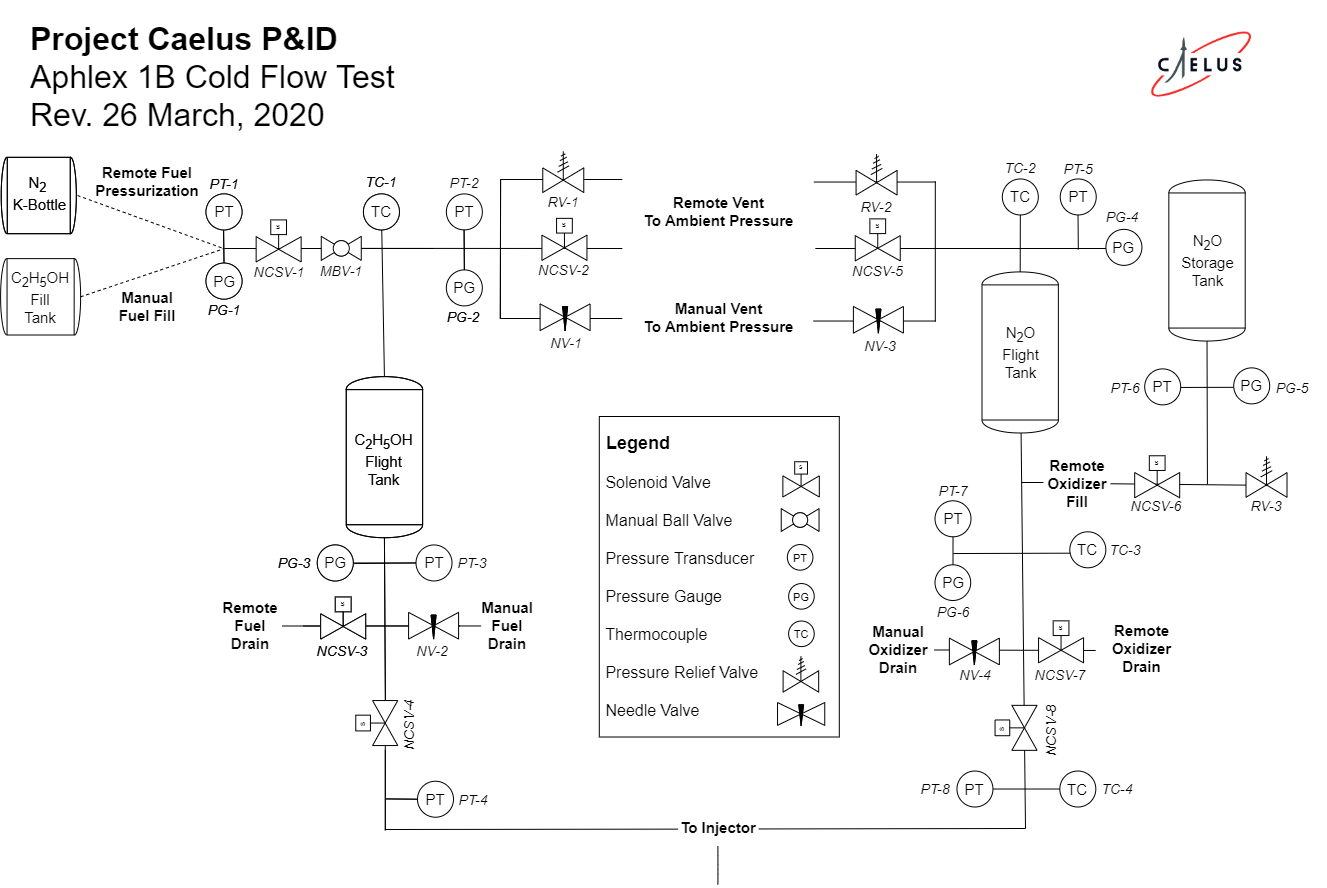
\includegraphics[scale=0.5, width=0.4\textwidth, trim={0cm 0cm 0cm 5cm}, clip]{pid} %L, B, R, T
    \caption{Full System Piping and Instrumentation Diagram}
    \label{fig:piping_and_instrumentation_diagram}
\end{figure}

\subsection{Ethanol Propellant Tower Plumbing}

\subsubsection{Ethanol Fill System}
\hspace{\parindent} Gravity fill was chosen for ethanol as it avoids the use of expensive or complicated pumps, making it a simple and cost-effective solution. First, ethanol will be poured manually into the tank since it is safe and not toxic, cryogenic, or at a high pressure where it might pose danger to someone manually handling it. During this time both MBV-1 and NCSV-1 will be open. Once this is complete, MBV-1 and NCSV-1 will be closed and the nitrogen K-bottle will be attached at this port to the rest of the piping system. This system is displayed in Figure \ref{fig:ethanol_fill_and_pressurization_system}.

\subsubsection{Ethanol Nitrogen Blowdown Pressurization System}
\hspace{\parindent} Pressure blowdown was chosen as the method of pressurization due to its simplicity along with a few other benefits. For example, in a rocket launch the utilization of pressure blowdown would allow the pressurant tank to remain on the ground (disconnection via quick disconnects and pneumatic actuators), which would significantly lower the GLOW of the rocket. Additionally, the large ullage percentage of the propellant run tank and short engine burn time would decrease the potential benefits of a pressure-regulated system. The nitrogen for the pressure blowdown will be a K-bottle with 2,000 PSI nitrogen.

To describe procedures, NCSV-1 will be remote-operated for control of pressurant flow, while MBV-1 is the isolation valve to ensure that pressurant is not unintentionally released when engineers are near the test stand. PT-1 and PG-1 will provide data on the pressurant tank pressure. Once ethanol has been filled, the nitrogen K-bottle has been properly connected, and all other checks are completed, the nitrogen K-bottle valve will be opened and PT-1 and PG-1 will start reading pressurant pressure data. Finally, MBV-1 will be opened at this time and all personnel will leave the test stand area and return to the team's safety bunker. NCSV-1 will then be opened remotely, allowing nitrogen from the K-bottle to flow into the tank until the tank is pressurized to the proper pressure. This system is displayed in Figure \ref{fig:ethanol_fill_and_pressurization_system}.

\begin{figure}[!htb] 
    \centering
    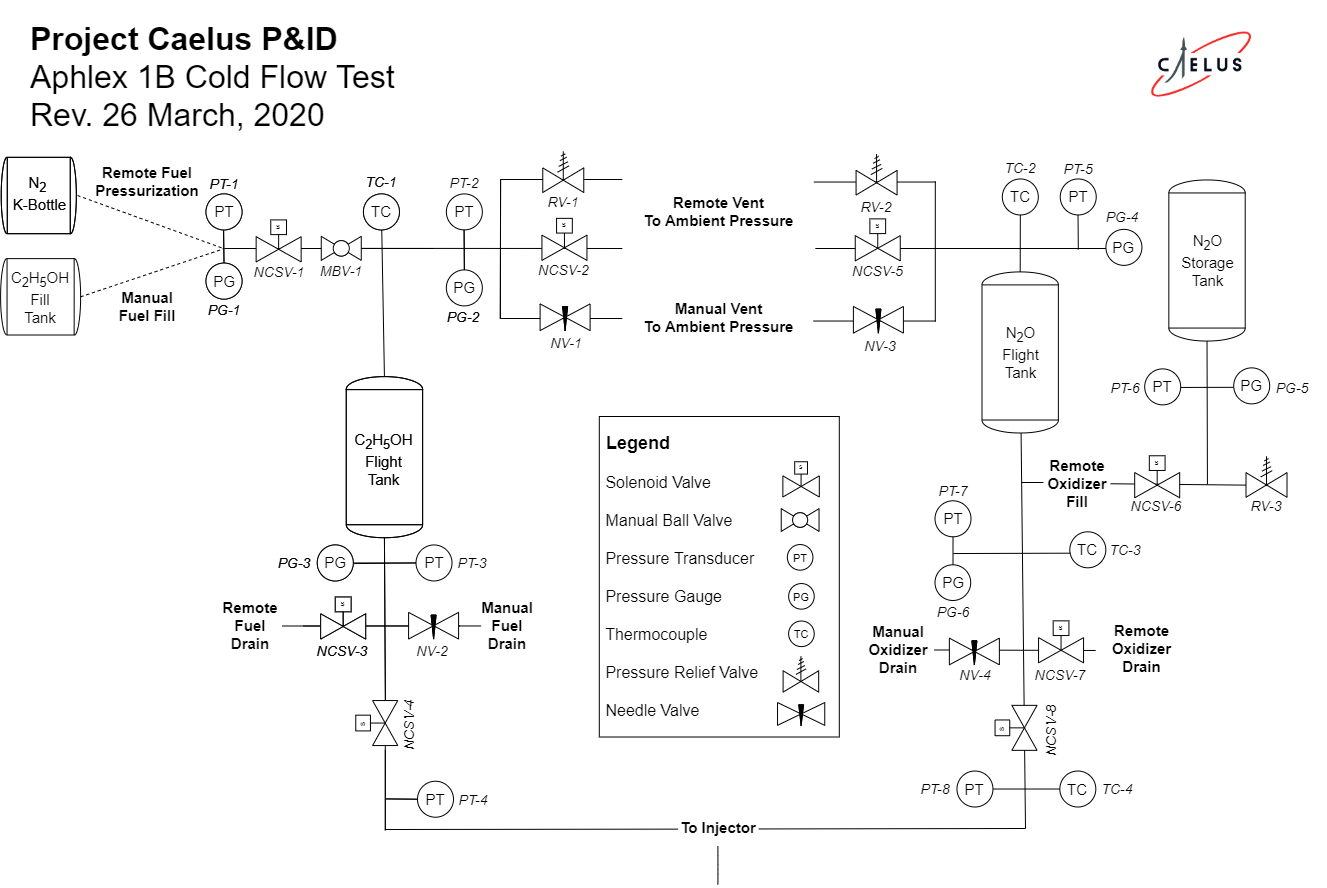
\includegraphics[scale=0.5, width=0.5\textwidth, trim={0cm 19cm 34.05cm 5cm}, clip]{pid} %L, B, R, T
    \caption{Ethanol Fill and Nitrogen Blowdown Pressurization System}
    \label{fig:ethanol_fill_and_pressurization_system}
\end{figure}

\subsubsection{Ethanol Pressure Vent System}
\hspace{\parindent} The ethanol pressure vent system consists of 3 main valves. The first of these, RV-1, a pressure relief valve, will be automatically set to open if tank pressure increases to above 600 PSI, which is about 50\% greater than would be nominally expected. The second valve, NCSV-2, a solenoid valve, will be remotely opened for small pressure vents, in the case of a failure with RV-1, or a full system abort. Finally, NV-1, a needle valve, will be used for any manual draining purposes as a last and to slowly ease tank pressure once the solenoids and pressure relief valves have dumped pressure adequately enough that engineers can safely approach the test stand. This system implements redundancy (RV-1 and NCSV-2) to ensure that there is always a back-up to relieve tank pressure when it is necessary even if a valve fails. This system is displayed in Figure \ref{fig:ethanol_vent_system}.

\begin{figure}[!htb] 
    \centering
    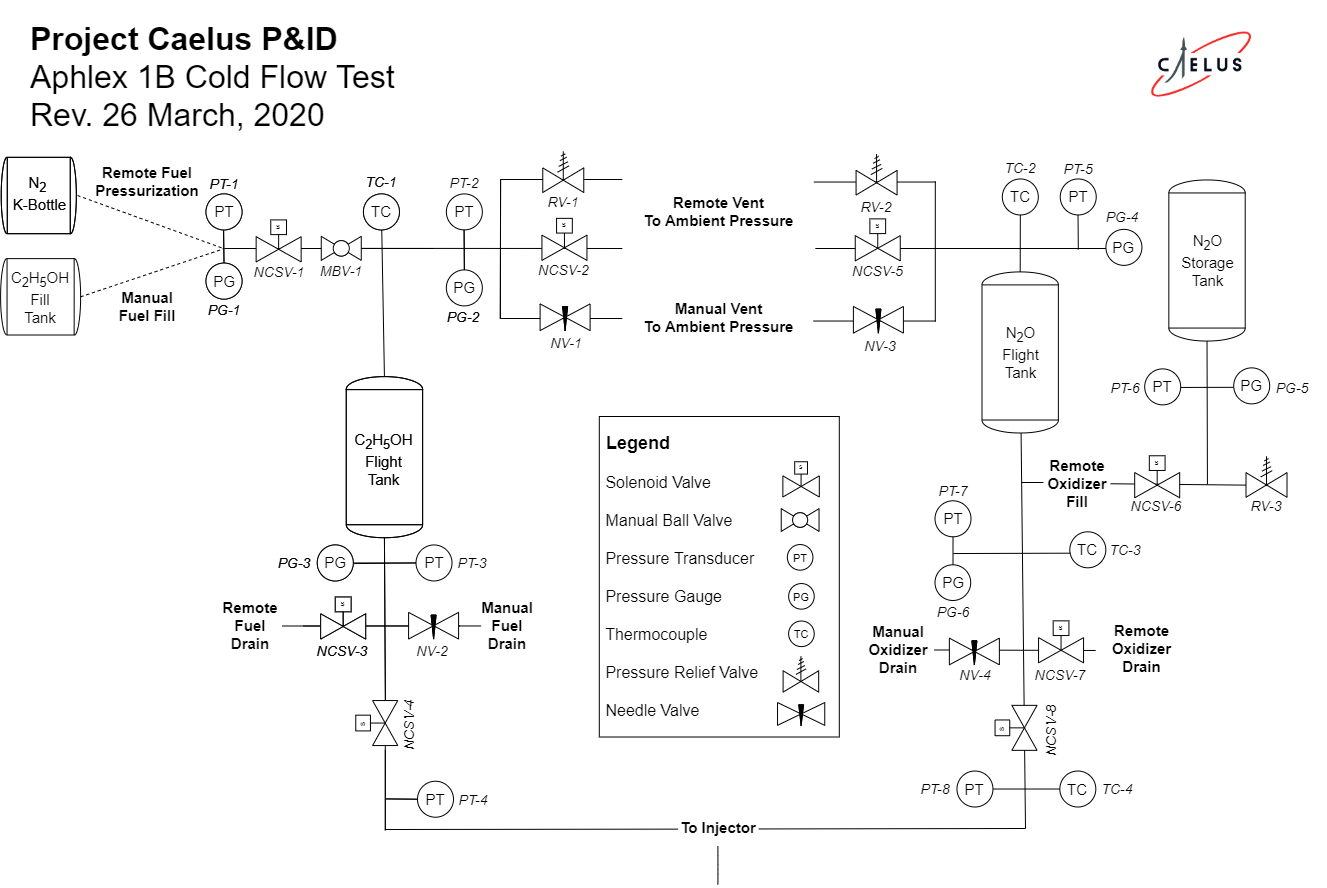
\includegraphics[scale=0.5, width=0.5\textwidth, trim={15cm 18cm 18.3cm 5cm}, clip]{pid} %L, B, R, T
    \caption{Ethanol Vent System}
    \label{fig:ethanol_vent_system}
\end{figure}

\subsubsection{Ethanol Drain System}
\hspace{\parindent} The ethanol system consists of two valves for drainage. The first is NCSV-3, a remotely-operated solenoid, which wil be used for most draining purposes, particularly in the case of a system abort. The second valve is NV-2, a manually-operated needle valve, which will serve as a way of draining propellant manually when the tank's pressure has adequately relieved. This system is displayed in Figure \ref{fig:ethanol_drain_system}.

\begin{figure}[!htb] 
    \centering
    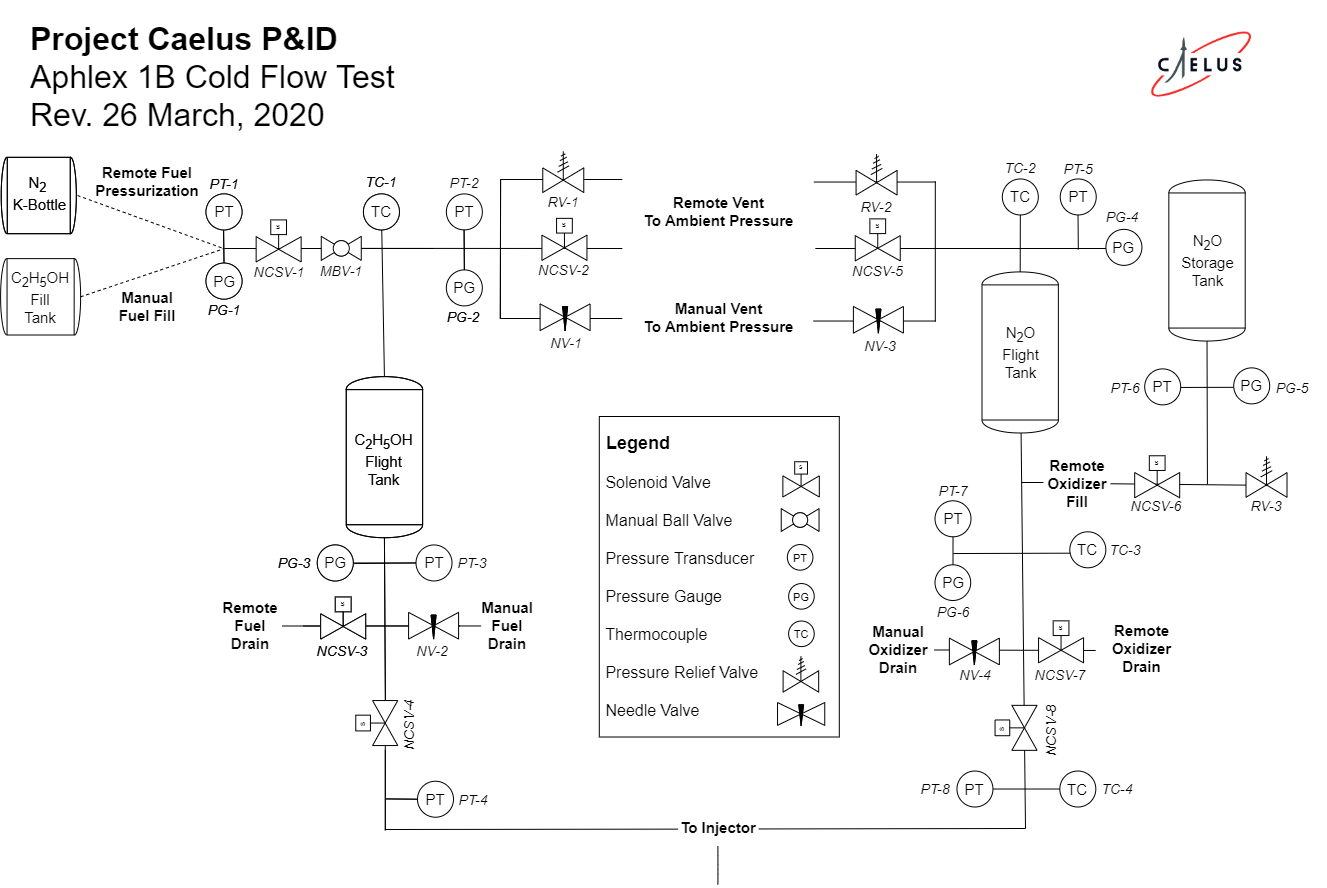
\includegraphics[scale=0.5, width=0.5\textwidth, trim={7cm 7cm 28cm 19.2cm}, clip]{pid} %L, B, R, T
    \caption{Ethanol Drain System}
    \label{fig:ethanol_drain_system}
\end{figure}

\subsection{Nitrous Oxide Propellant Tower}
\subsubsection{Nitrous Oxide Fill System}
\subsubsection{Nitrous Oxide Self-Pressurization System}
\subsubsection{Nitrous Oxide Vent System}
\subsubsection{Nitrous Oxide Drain System}

\section{Ethanol Cold Flow Test Stand Design}
\hspace{\parindent} The ethanol cold flow test will entail running water through the full ethanol propellant tower, as well as through the injector and into the engine. The main reasons for this test include empirically verifying theoretical calculations and pressure drops, verifying system integrity, and ensuring that all programming procedures function nominally. Most importantly, this will be the first major hardware test and will test procedures for assembly, leak-checking, filling, pressurization, draining, data-collection, valve control, and aborting.

This test will be run in two different ways: at full pressure and at scaled pressure, each of which will provide different valuable information and procedural practice to progress towards a static hot fire of the engine.

A full pressure cold flow test involves pressurizing the tank to the pressure it will be at during an actual fire, and this is to test the pressure rating of all parts of the system such as valves and sensors, and stress testing the system to verify performance levels. Furthermore this can be used to ensure that this system can safely operate at it's normal working pressure, including whether pressure can be properly relieved in the case of an abort.

Scaled pressure, however, is making the pressure differential between the tank and chamber equal to the actual differential we will be expecting in the static fire. Since there will be no combustion in the chamber, it's pressure will be at 1 atm. This is much lower than the actual combustion chamber temperature and would therefore result in a higher mass flow rate if our tank pressure remained the same. By properly scaling down our tank pressure, it would be possible to accurately measure the system Cv, as well as to determine mass flow rate and tank pressure depletion profile over time.

To accomplish these goals, the plumbing detailed in section 4.1 must be fully constructed as a test stand, along with a separate injector and engine mechanism which could later be used to measure thrust in an actual static fire. The following subsections will detail these two major parts of the test stand for this test.
\subsection{Tank Stand and Plumbing}
\hspace{\parindent} The tank stand and plumbing had to contain the ethanol flight tank, nitrogen K-bottle for pressurization, and all the plumbing up until the engine. The design for this test stand included a frame of aluminum 80/20s which would hold the ethanol flight tank in place, as well as cinder blocks as a stand for the temporary nitrogen K-bottle. The plumbing will mostly be bolted to a 1/8" thick steel plate on the outside of the 80/20 steel frame for the ethanol tank. This will allow for all plumbing to be easily accessible for small changes or for turning manual valves, as well as for pressure gauges to be monitored via video camera live stream in the event of a pressure transducer failure. A rendering of the ethanol tower tank stand and plumbing section is shown in Figure \ref{fig:ethanol_tank_stand_render}.

\begin{figure}[!htb] 
    \centering
    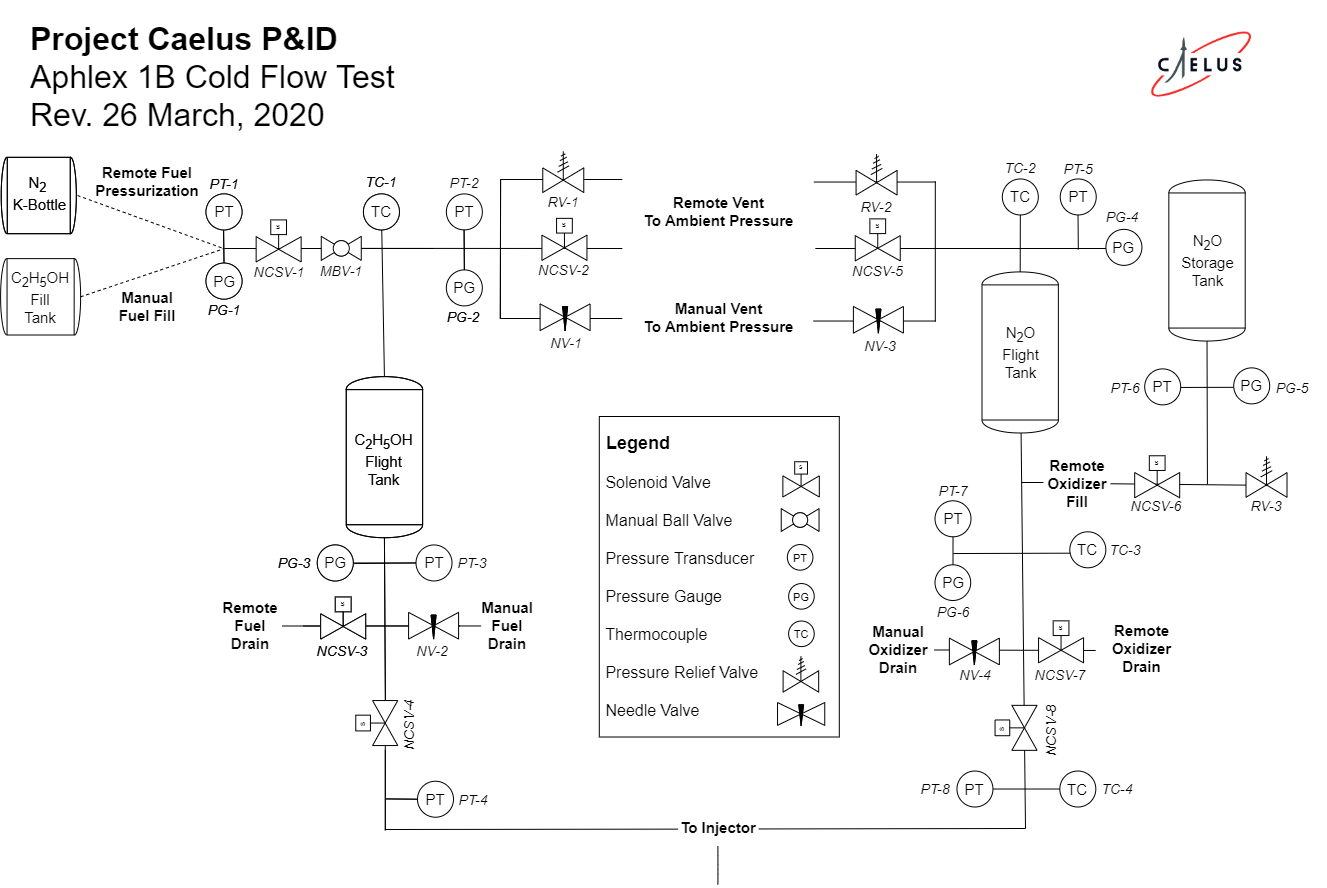
\includegraphics[scale=0.5, width=0.5\textwidth]{pid} %L, B, R, T
    \caption{Ethanol Propellant Tower Test Stand Render}
    \label{fig:ethanol_tank_stand_render}
\end{figure}

\subsection{Engine and Injector}

\section{Parts and Budget}

% \section{Nitrous Oxide Cold Flow Test Stand Design}
% \section{Full Test Stand Design}
% \section{Launch Vehicle Design}
% \subsection{Objectives}
% \subsection{Callisto 1}

\printbibliography
% To compile bibliography, run pdfLaTeX ONLY, then Biber, then pdfLaTeX ONLY
%\end{multicols}

\end{document}
